\documentclass{report}
\usepackage{fullpage,amssymb,amsmath,graphicx,tabularx,rotating,spverbatim}
%\usepackage[euler]{textgreek} %define \textmu

\usepackage{siunitx}
\sisetup{range-phrase=--, , range-units=single}
\usepackage[version=4]{mhchem}

\usepackage{lmodern}

%\usepackage[utf8]{inputenc}
%\usepackage[english]{babel}
\usepackage[hidelinks]{hyperref}
\usepackage[nottoc]{tocbibind}
\usepackage[toc,page]{appendix}

\usepackage[backend=biber,style=ieee,citestyle=numeric,sorting=none]{biblatex}
\addbibresource{co2amp.bib}

\begin{document}

\title{co2amp}
\author{Mikhail Polyanskiy}

\date{2024-11-01}
\maketitle

\tableofcontents

%%%%%%%%%%%%%%%%%%%%%%%%%%%%%%%%%%%%%%%%%%%%%%%%%%%%%%%%%%%%%%%%%%%%%%%%%%%%%%%%%
%%%%%%%%%%%%%%%%%%%%%%%%%%%%%%%%%%%%%%%%%%%%%%%%%%%%%%%%%%%%%%%%%%%%%%%%%%%%%%%%%
%%%%%%%%%%%%%%%%%%%%%%%%%%%%%%%%%%%%%%%%%%%%%%%%%%%%%%%%%%%%%%%%%%%%%%%%%%%%%%%%%
\chapter{General notes}

\section{Program Capabilities}
\begin{enumerate}
    \item Ultrashort pulse amplification in \ce{CO2} active medium
    \begin{itemize}
        \item Rotational numbers up to \( J = 60 \)
        \item Regular, hot, and sequence bands
        \item Isotopic \ce{CO2}
    \end{itemize}
    \item Molecular dynamics
    \begin{itemize}
        \item Realistic pumping
        \item Collisional relaxation processes
        \item Stimulated transitions
        \item Independent consideration of active medium regions at different elongations from the optical axis
    \end{itemize}
    \item Diffraction-based beam propagation
    \begin{itemize}
        \item Beam manipulation with common optical elements
        \item Arbitrary optical configurations
    \end{itemize}
    \item Linear dispersion and non-linear effects in optical materials
    \begin{itemize}
        \item Pulse chirping
        \item Kerr lensing
        \item Self-phase modulation
    \end{itemize}
    \item Advanced optics
    \begin{itemize}
        \item Chirped-pulse amplification
        \item Spectral filtering
        \item Trains of pulses
        \item Staging (program output as an input for the next stage)
    \end{itemize}
    \item User's interface
    \begin{itemize}
        \item Easy specification of parameters
        \item Graphical output
        \item Project save/recall
    \end{itemize}
\end{enumerate}


\section{Availability, Tools, and Third Party Components}
The simulation core \textbf{\texttt{co2amp}} and the user's interface shell \textbf{\texttt{co2amp+}} are written in the C++ programming language. \textbf{\texttt{co2amp+}} utilizes the \texttt{QT} library (\url{http://qt.io}), and \texttt{QT Creator}, a component of the \texttt{QT} project, is employed as the development environment. Windows executables are compiled using the \texttt{MinGW} compiler, which is part of the open-source \texttt{QT} distribution. The code is hosted on GitHub (\url{https://github.com/polyanskiy/co2amp}) and is freely available for use, modification, and redistribution under the GNU General Public License (GPL v.3) (\url{https://www.gnu.org/licenses/gpl-3.0.html}). A binary package is available as a Windows installer, containing pre-compiled executables, documentation, templates, and examples at \url{https://github.com/polyanskiy/co2amp/releases/}. The project leverages cross-platform libraries, facilitating compilation on other platforms (MacOS, Linux). \textbf{\texttt{co2amp}} relies on three third-party components: \texttt{gnuplot}, \texttt{7-zip}, and \texttt{HDF5}, available at \url{http://www.gnuplot.info/}, \url{https://www.7-zip.org/}, and \url{https://www.hdfgroup.org/solutions/hdf5/}, respectively. These components must be installed separately. The Windows installer is created using the \texttt{Nullsoft Scriptable Install System (NSIS, \url{https://nsis.sourceforge.io/})}, representing the only platform-specific component of the project. The documentation is primarily written in \LaTeX (\url{http://www.latex-project.org}) using the \texttt{Overleaf} online editor and compiler (\url{https://www.overleaf.com/}). YAML and HDF5 file formats are adopted for specifying input parameters and storing output field information, respectively.



\section{Acknowledgements}
Viktor Platonenko from Moscow State University (Russia) provided a \texttt{Mathcad} code for pulse amplification in the \ce{CO2} active medium, which served as the starting point for developing the \textbf{\texttt{co2amp}} program. Dr.~Platonenko also offered valuable input during the early stages of the work on \textbf{\texttt{co2amp+}}.



%%%%%%%%%%%%%%%%%%%%%%%%%%%%%%%%%%%%%%%%%%%%%%%%%%%%%%%%%%%%%%%%%%%%%%%%%%%%%%%%%
%%%%%%%%%%%%%%%%%%%%%%%%%%%%%%%%%%%%%%%%%%%%%%%%%%%%%%%%%%%%%%%%%%%%%%%%%%%%%%%%%
%%%%%%%%%%%%%%%%%%%%%%%%%%%%%%%%%%%%%%%%%%%%%%%%%%%%%%%%%%%%%%%%%%%%%%%%%%%%%%%%%
\chapter{Basic Concepts}

%%%%%%%%%%%%%%%%%%%%%%%%%%%%%%%%%%%%%%%%%%%%%%%%%%%%%%%%%%%%%%%%%%%%%%%%%%%%%%%%%
\section{\textbf{\texttt{co2amp}} and \textbf{\texttt{co2amp+}}}
\textbf{\texttt{co2amp}} is a terminal program designed for simulating the propagation of ultrashort pulses through an arbitrary cylindrically-symmetric optical system, which may include \ce{CO2} amplifiers. It operates using inputs in the form of specially formatted text files and command line arguments, and generates outputs as tabulated data files and a binary file containing comprehensive information on the output field. While \textbf{\texttt{co2amp}} can function independently, its use is greatly facilitated by a graphical user interface, which significantly simplifies the management of the program’s inputs and outputs.

\textbf{\texttt{co2amp+}} is a graphical user interface program that streamlines the process of handling multiple input and output files, as well as calculation parameters, by maintaining an organized and easily navigable working environment. \textbf{\texttt{co2amp+}} features functionality for saving and recalling the entire file structure of a project along with command line parameters in a single compressed '.co2' file.


%%%%%%%%%%%%%%%%%%%%%%%%%%%%%%%%%%%%%%%%%%%%%%%%%%%%%%%%%%%%%%%%%%%%%%%%%%%%%%%%%
\section{Projects}
The \textbf{\texttt{co2amp}} input parameters include the characteristics of the initial \texttt{pulse(s)}, the optical \texttt{layout} configuration, specifications for all \texttt{optics} used in the model (including laser amplifiers), and calculation parameters (e.g., calculation grid definition).

The temporal shape of the pulse and the beam profile at every element of the optical layout are saved and can be accessed in both graphical and tabulated-numerical representations.

All \textbf{\texttt{co2amp}} inputs and outputs for a certain model constitute a project.

\textbf{\texttt{co2amp+}} facilitates the storage of all inputs and outputs of the model, except for the output field, in a single compressed project file with a '.co2' extension. Complete pulse information (complex field at every node of the space-time calculation grid) at the system's output can be saved separately as a binary HDF5 file (with a '.pulse' extension) and used as an input for another project. An example of the input file structure of a '.co2' project accessed via the \textbf{\texttt{co2amp+}} interface is illustrated in Fig.~\ref{fig:gui-input}.

\begin{figure}[ht]
 \centering
 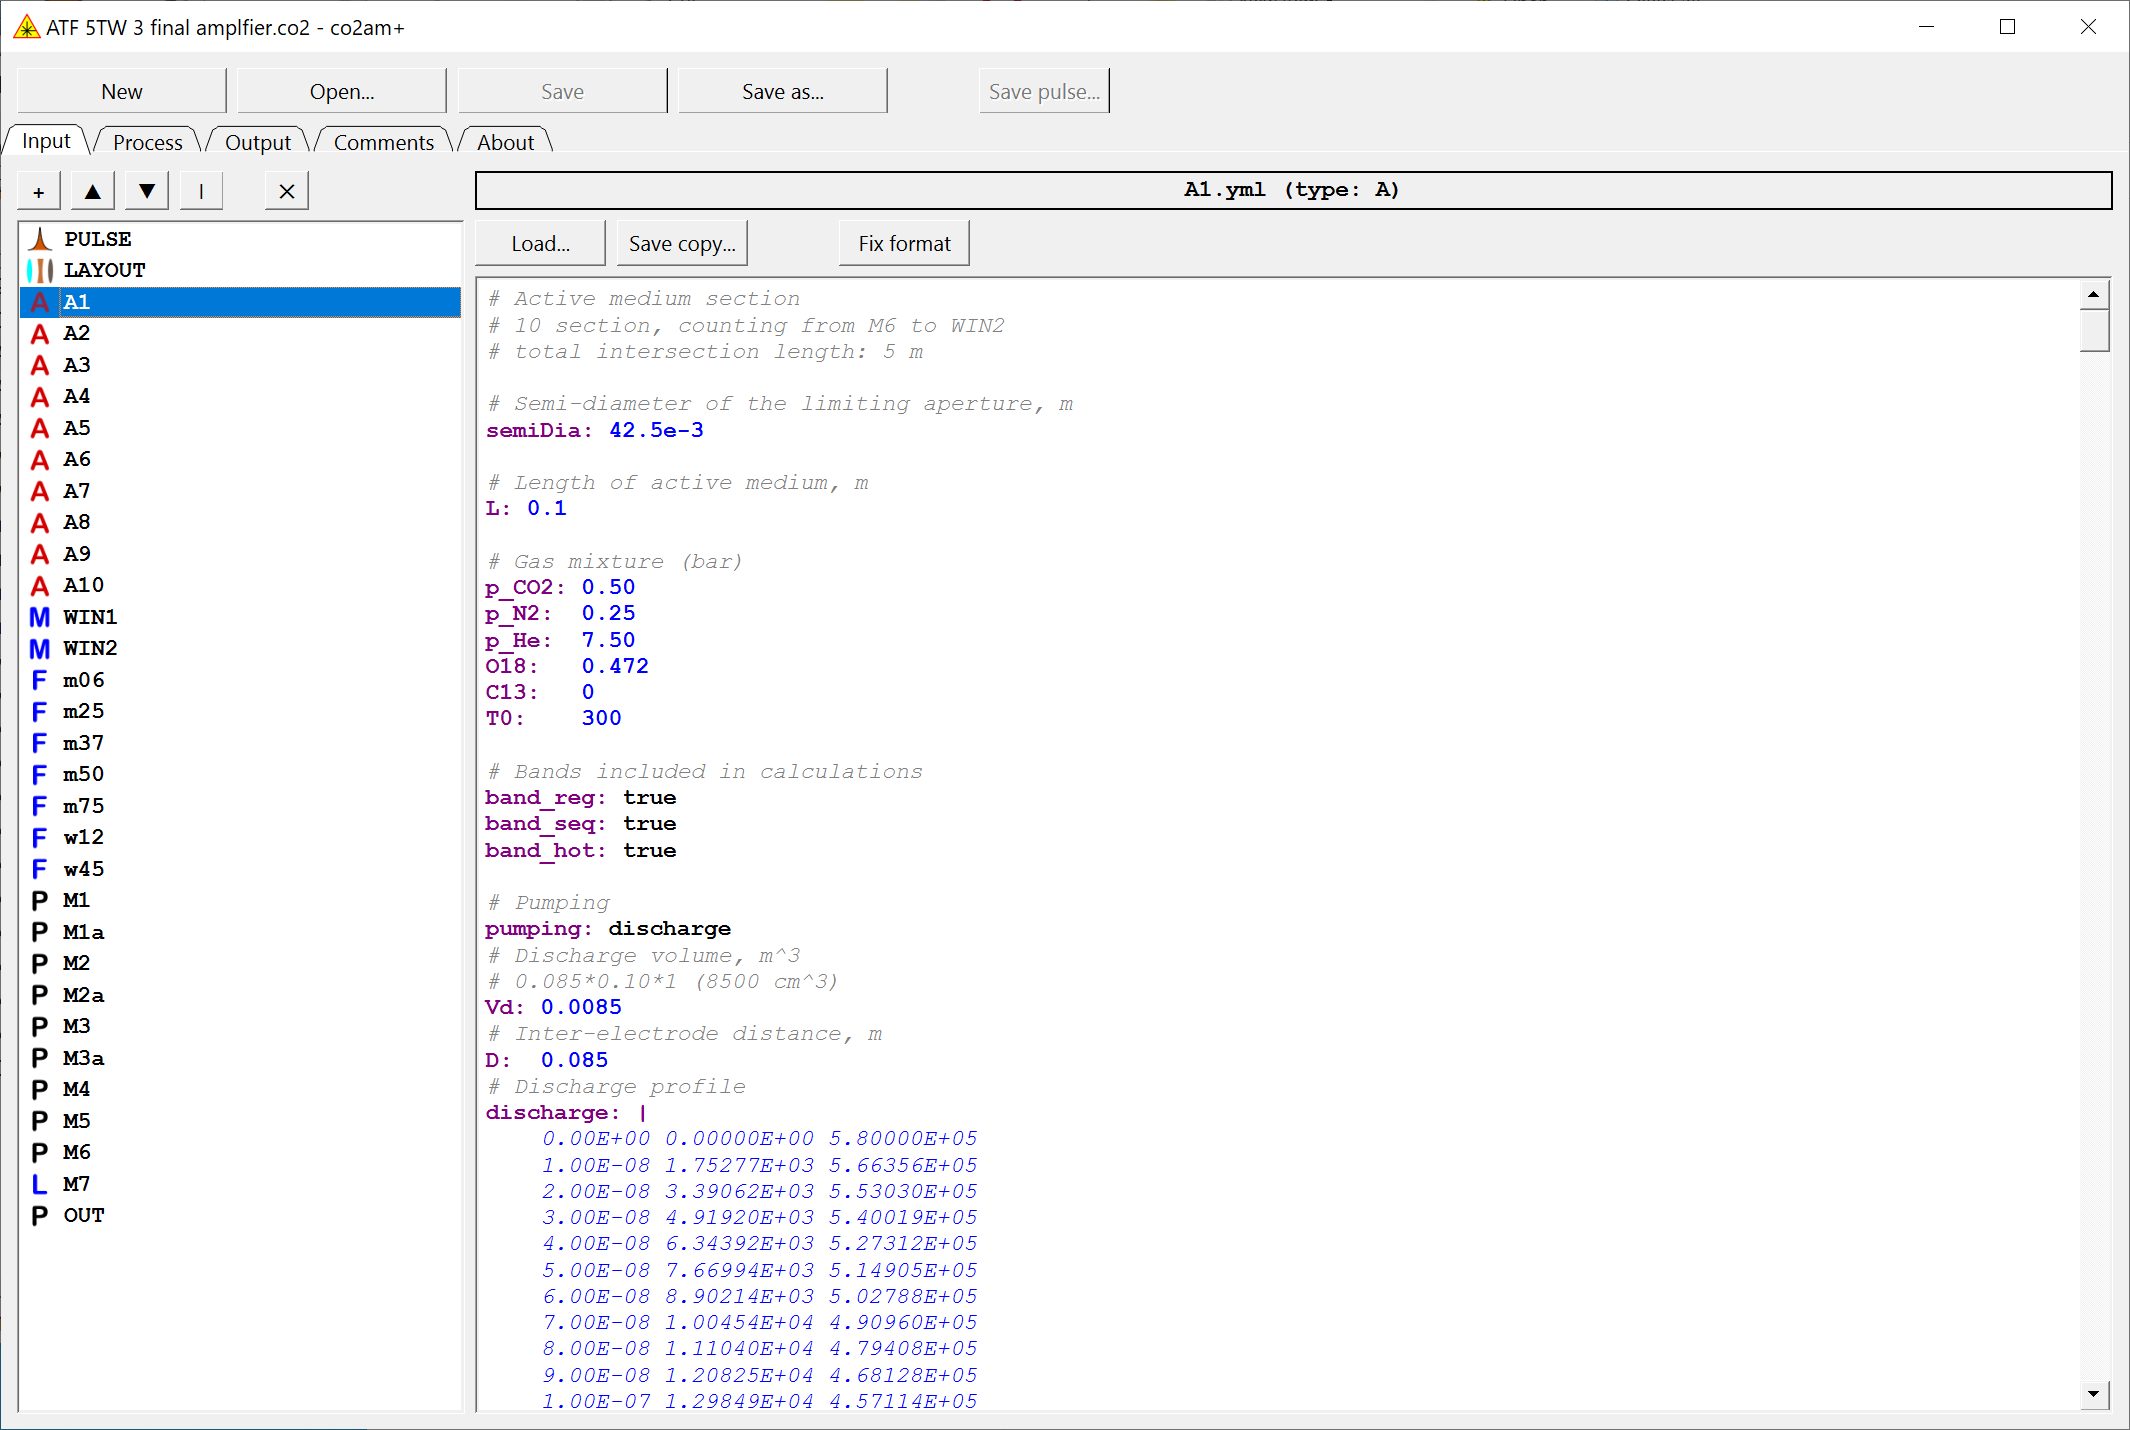
\includegraphics[width=14cm]{images/gui-input}
 \caption{"Input" tab of the \textbf{\texttt{co2amp+}} user interface program. YAML files specifying the \texttt{pulse}, \texttt{layout}, and \texttt{optics} are listed on the left. Content of a selected file is displayed and can be edited in the big edit box on the right.}
 \label{fig:gui-input}
\end{figure}


%%%%%%%%%%%%%%%%%%%%%%%%%%%%%%%%%%%%%%%%%%%%%%%%%%%%%%%%%%%%%%%%%%%%%%%%%%%%%%%%%
\section{\texttt{Pulse}, \texttt{Layout} and \texttt{Optic}}
A \texttt{pulse} is a complex electric field defined at every node of the calculation grid. A project can include one or more input pulses. Each is defined in a separate YAML ('.yml') file. A pulse can be defined either by referencing an output from another project (a '.pulse' file) or by explicitly specifying the pulse's spatial and temporal profile.

The optical \texttt{layout} consists of a series of infinitely-thin \texttt{optics} separated by free space. \texttt{Pulses} propagate freely between \texttt{optics}. A project must have exactly one \texttt{layout}. The \texttt{layout} is defined in a '.yml' file that specifies the order of the \texttt{planes} and the distances between them.

An \texttt{optic} is a system element that alters the pulse as it passes through. Several types of \texttt{optics} are described in detail later. For example, a \textit{Lens} is an \texttt{optic} introducing a radial-coordinate-dependent frequency shift, altering the beam's divergence. Each \texttt{optic} is specified in a separate '.yml' file. An \texttt{optic} can be used multiple times in the same \texttt{layout}, as in a laser cavity\footnote{Internally, the \textbf{\texttt{co2amp}} code employs an additional concept: a \texttt{plane}. A \texttt{plane} is a \texttt{layout} element that, unlike an \texttt{optic}, appears in the \texttt{layout} only once. An \texttt{optic} is then associated with each \texttt{plane}. Essentially, a \texttt{plane} is a placeholder for an \texttt{optic}.}.

\textbf{\texttt{co2amp}} supports seven types of \texttt{optics}, listed in Table~\ref{table:optics}.

\begin{table}
\caption{Types of \texttt{Optics}}
\label{table:optics}
\begin{tabularx}{\textwidth}{c l X}
\hline 
\textit{\textbf{Type ID}} & \textit{\textbf{Name}} & \textit{\textbf{Description}}\\
\hline 
&&\\
A & \textit{Active medium} & A CO$_2$ amplifier section.\\
&&\\
P & \textit{Probe} & A passive surface. May be used as a limiting aperture.\\
&&\\
F & \textit{Spatial filter} & An \texttt{optic} with coordinate-dependent transmission.\\
&&\\
S & \textit{Spectral filter} & An \texttt{optic} with frequency-dependent transmission.\\
&&\\
L & \textit{Lens} & An ideal thin lens.\\
&&\\
M & \textit{Material} & A layer of material. May introduce linear and/or non-linear dispersion and/or absorption.\\
&&\\
C & \textit{Chirper} & An \texttt{optic} that applies a chirp to the pulse. Typically a stretcher or compressor.\\
\hline
\end{tabularx}
\end{table}


%%%%%%%%%%%%%%%%%%%%%%%%%%%%%%%%%%%%%%%%%%%%%%%%%%%%%%%%%%%%%%%%%%%%%%%%%%%%%%%%%
\section{Calculation Grid}
The \texttt{pulse} is defined as a complex electric field at the nodes of a 2-dimensional space-time calculation grid, which moves with the pulse. The calculation grid is primarily defined via \textbf{\texttt{co2amp}} command line arguments. The only exception is the maximum radial coordinate, equal to the semi-diameter of the clear aperture of an \texttt{optic}, and thus varies from one \texttt{optic} to another. The command line arguments associated with the pulse's space-time calculation grid include the numbers of nodes (representing "precision") in the time and radial coordinate grids, the minimum and maximum time limits, and the central frequency. The central frequency is essential for unambiguously defining the calculation grid in the frequency domain.

The pulse time frame is utilized for all \texttt{pulse}-related calculations (interaction with \texttt{optics}, free-space propagation) and for fast processes in some \texttt{optics}, such as fast molecular dynamics (stimulated transitions and rotational relaxation in an \textit{Active Medium}). Processes significantly slower than the pulse duration (like the pumping of the active medium and vibrational relaxation) are modeled separately in a slower laboratory time-frame. The time-tick of this laboratory time-frame is also defined via a \textbf{\texttt{co2amp}} command line argument.

In \textbf{\texttt{co2amp+}}, the \textbf{\texttt{co2amp}} command line arguments are specified in the "Process" tab (Fig.~\ref{fig:gui-process}).
\begin{figure}[ht]
 \centering
 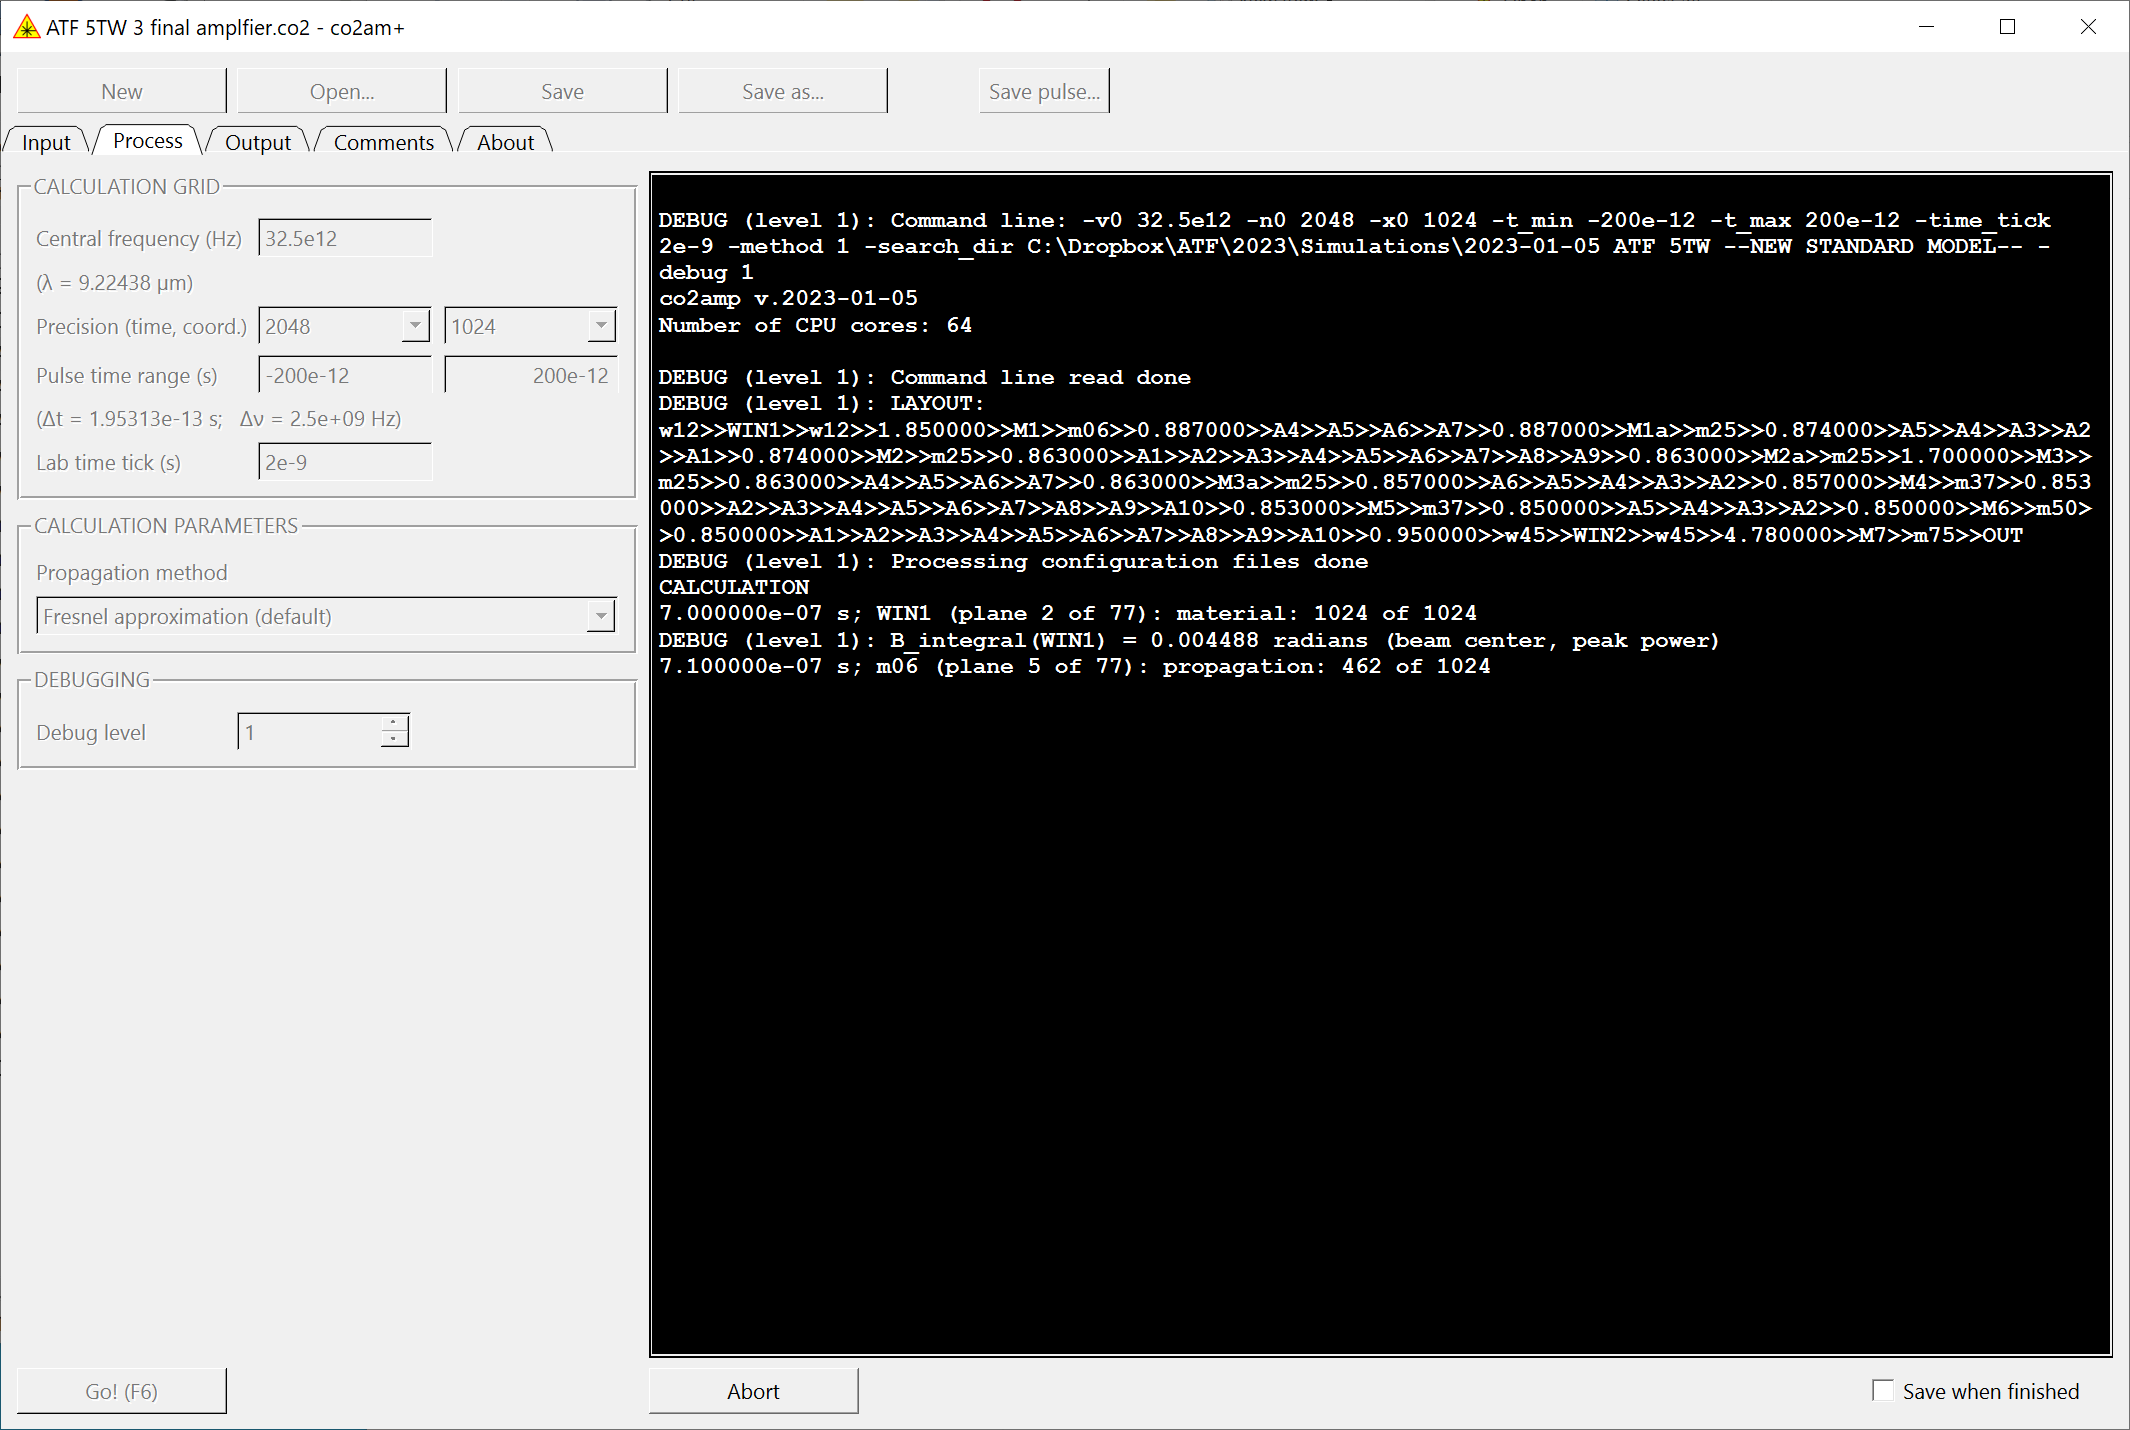
\includegraphics[width=14cm]{images/gui-process}
 \caption{"Process" tab of the \textbf{\texttt{co2amp+}} user interface program. Values of \textbf{\texttt{co2amp}} command line arguments are specified on the left. \textbf{\texttt{co2amp}} output is displayed in the black text box on the right.}
 \label{fig:gui-process}
\end{figure}
The number of nodes in both coordinates of the pulse space-time frame is always a power of two, enabling the use of Fast Fourier Transform (FFT) algorithms. Calculations with more nodes are generally more accurate but require longer computation times and more computer memory (both calculation time and required memory are approximately proportional to the product of the number of nodes in the time and space grids). Therefore, it is recommended to start the simulation with a smaller number of nodes and incrementally increase the grid density, repeating the simulation multiple times. The absence of significant changes in the program’s output with an increase in the number of nodes indicates that the grid density is satisfactory.

The time-step, \( \Delta t = (t_{\text{max}} - t_{\text{min}}) / N_t \), where \( t_{\text{max}} \) and \( t_{\text{min}} \) define the time range and \( N_t \) is the number of nodes in the time grid, must be sufficiently small to accurately describe the pulse profile throughout its propagation in the optical system. It is also important to note that the time range and the number of nodes in the time grid define the frequency domain range and step: \( \Delta\nu = 1 / (t_{\text{max}} - t_{\text{min}}) \) and \( (\nu_{\text{max}} - \nu_{\text{min}}) = 1 / \Delta t \). This means that the time range must be long enough to provide adequate resolution in the frequency domain, while the time step must be short enough to encompass the entire spectral region of interest.

Identifying an appropriate calculation grid is crucial for building an accurate model of an optical system. Investing effort in this part of the simulation process will yield fast and reliable calculations.


%%%%%%%%%%%%%%%%%%%%%%%%%%%%%%%%%%%%%%%%%%%%%%%%%%%%%%%%%%%%%%%%%%%%%%%%%%%%%%%%%
\section{Units}
SI units without prefixes, such as "meters, seconds, Amperes" (but not "centimeters, nanoseconds, kiloamperes"), are used in \textbf{\texttt{co2amp}} for input, output, and also internally within the code. \textbf{\texttt{co2amp+}} provides the functionality to change the units used for graphical representation of the calculation results on the "Output" tab (Fig.~\ref{fig:gui-output}).
\begin{figure}[ht]
 \centering
 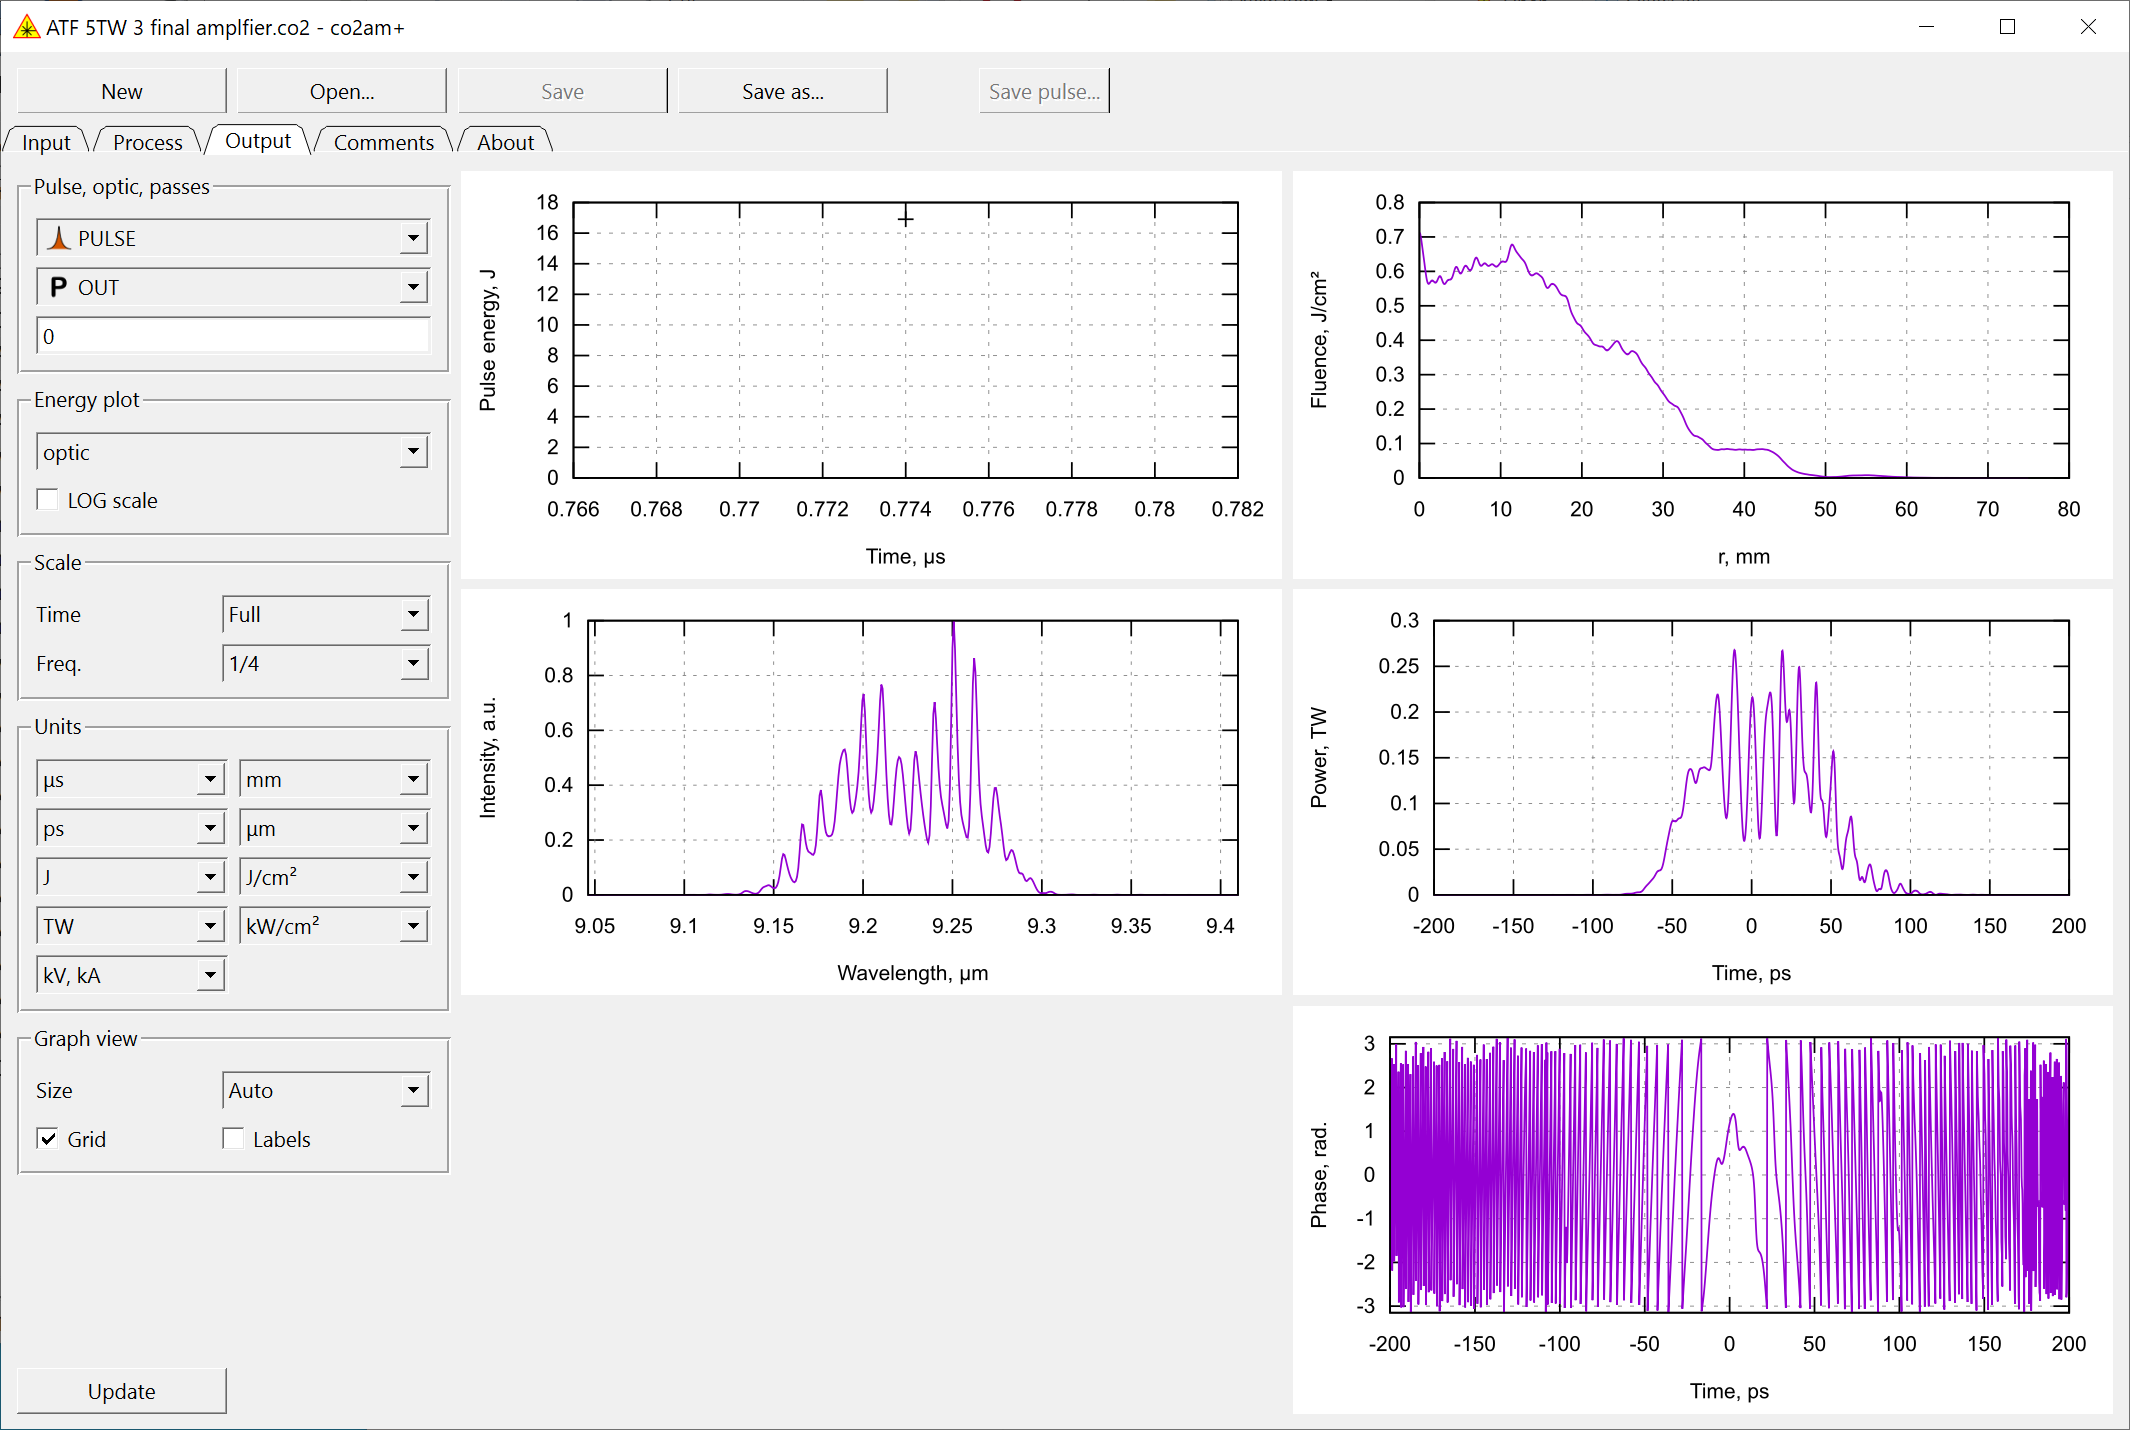
\includegraphics[width=14cm]{images/gui-output}
 \caption{"Output" tab of the \textbf{\texttt{co2amp+}} user interface program. Controls on the left allow selecting the data to display and fine-tuning the look of the plots.}
 \label{fig:gui-output}
\end{figure}
However, when numerical data are accessed via [Right-click on a plot] -- [Copy raw data], the units of the data are always in their "prefix-less" form.


%%%%%%%%%%%%%%%%%%%%%%%%%%%%%%%%%%%%%%%%%%%%%%%%%%%%%%%%%%%%%%%%%%%%%%%%%%%%%%%%%
\section{Program Output}
The output of the program includes the temporal and spatial structure of each \texttt{pulse} at every \texttt{optic} within the \texttt{layout}. Temporal (and spectral) profiles are integrated over the entire area of the \texttt{optic}, while spatial profiles are integrated over the duration of the pulse time-frame.

In the \textbf{\texttt{co2amp+}} "Output" tab, users can choose a \texttt{pulse} and an \texttt{optic} to display (Fig.~\ref{fig:gui-output}). If the selected \texttt{optic} is utilized multiple times in the \texttt{layout}, there is also an option to specify which passes through the \texttt{optic} are to be displayed. Additionally, the integral pulse energy can be provided either at each pass through a selected \texttt{optic} or across all passes through all \texttt{optics} in the \texttt{layout}.

Output for certain types of \texttt{optics} includes additional type-specific information. For example, for an \textit{Active medium}, this encompasses gain, discharge profile, population dynamics, and the dynamics of the distribution of pumping energy (fractions of discharge energy contributing to the excitation of laser levels, excitation of molecular translations, and ionization). Output for an \texttt{optic} of type \textit{Probe} includes information on the phase of the optical field at the center of the beam.


%%%%%%%%%%%%%%%%%%%%%%%%%%%%%%%%%%%%%%%%%%%%%%%%%%%%%%%%%%%%%%%%%%%%%%%%%%%%%%%%%
\section{"Comments" and "About" Tabs of \textbf{\texttt{co2amp+}}}
The "Comments" tab in \textbf{\texttt{co2amp+}} provides an editable text box where users can enter any comments about the project. These comments will be stored as part of the project in the '.co2' file.

The "About" tab contains information about the versions of \textbf{\texttt{co2amp}} and \textbf{\texttt{co2amp+}}, including links to the license and the documentation (this file), author contact information, and a suggested citation format.


%%%%%%%%%%%%%%%%%%%%%%%%%%%%%%%%%%%%%%%%%%%%%%%%%%%%%%%%%%%%%%%%%%%%%%%%%%%%%%%%%
%%%%%%%%%%%%%%%%%%%%%%%%%%%%%%%%%%%%%%%%%%%%%%%%%%%%%%%%%%%%%%%%%%%%%%%%%%%%%%%%%
%%%%%%%%%%%%%%%%%%%%%%%%%%%%%%%%%%%%%%%%%%%%%%%%%%%%%%%%%%%%%%%%%%%%%%%%%%%%%%%%%
\chapter{Elements of a Project}

A project in \textbf{\texttt{co2amp}} must include the following elements, each specified in separate input YAML ('.yml') files:
\begin{enumerate}
    \item One or more \texttt{pulses}
    \item One or more \texttt{optics}
    \item One \texttt{layout}
\end{enumerate}
Each element is detailed in its dedicated YAML file\footnote{\textbf{\texttt{co2amp}} additionally requires an input file 'config\_files.yml' that enumerates all input YAML files and the types of corresponding elements. \textbf{\texttt{co2amp+}} automatically generates this file.}. The last \texttt{optic} in the \texttt{layout} must be of type P (\textit{Probe}).

The subsequent sections provide brief descriptions of each of these elements and the models associated with them. For a comprehensive understanding, refer to the templates, example files, and the comments within them.


%%%%%%%%%%%%%%%%%%%%%%%%%%%%%%%%%%%%%%%%%%%%%%%%%%%%%%%%%%%%%%%%%%%%%%%%%%%%%%%%%
\section{\texttt{Pulse}}
Unless utilizing the output of another project (a '.pulse' file) as input, both the temporal and spatial shape of the input \texttt{pulse} must be defined in a corresponding YAML ('.yml') file. The \texttt{pulse} is assumed to be transform-limited, meaning it has no initial chirping. Specifications such as the \texttt{pulse} energy, central frequency, and injection time are also required. The injection time denotes the time-delay between the zero moment of the laboratory time frame ("slow" time frame) and the injection of a \texttt{pulse} into the optical system (the first \texttt{optic} in the \texttt{layout}). An example of a \texttt{pulse} configuration file is provided below.

\begin{verbatim}
#=========================
# PULSE.yml from 'examples/00 simple propagation.co2' project

t_in: 0
E: 1e-3
freq: 32.5e12

beam: GAUSS
w: 3e-3

pulse: GAUSS
fwhm: 2e-12
#=========================
\end{verbatim}

This file specifies a 2~ps (FWHM) transform-limited Gaussian pulse with a $w=3$~mm Gaussian beam profile, 1~mJ energy, and a 32.5~THz central frequency, injected into the system at $t_{\text{in}}=0$. Several pre-defined beam and pulse profile options are available, such as \texttt{GAUSS}, \texttt{FLATTOP}, \texttt{SUPERGAUSS4}, \texttt{SUPERGAUSS6}, etc. Alternatively, a \texttt{FREEFORM} option allows for the specification of an arbitrary shape through a tabulated numerical profile (refer to the 'pulse.yml' template for details).


%%%%%%%%%%%%%%%%%%%%%%%%%%%%%%%%%%%%%%%%%%%%%%%%%%%%%%%%%%%%%%%%%%%%%%%%%%%%%%%%%
\section{\texttt{Layout}}
\subsection{Configuration}
The \texttt{layout} configuration defines the sequence of \texttt{optics} and the distances between them in the optical system. Below is an example of a simple \texttt{layout} configuration file:

\begin{verbatim}
#=========================
# LAYOUT.yml from 'examples/00 simple propagation.co2' project

- go: P1 >> 3 >> P2
  times: 1
#=========================
\end{verbatim}

In this example, the system consists of two \texttt{optics}, \texttt{P1} and \texttt{P2}, separated by 3 meters of free space. The pulses pass through the system once. If the \texttt{times} value is greater than 1, a pulse after passing through \texttt{P2} will return to \texttt{P1}, and the propagation through the system will repeat for the specified number of times. A \texttt{layout} configuration file can contain several such "go-times" sequences. Below is an example of a \texttt{layout} configuration for a more complex system:

\begin{spverbatim}
#=========================
# LAYOUT.yml from 'examples/ATF 5 TW/ATF 1 regen.co2' project

- go: str >> COU1
  times: 1

- go: 0.45 >> i >> 0.90 >> GE >> 0.25 >> w >> WIN1 >> w >> 0.45 >> AM1 >> 0.40 >> AM2 >> 0.45 >> w >> WIN2 >> w >> 0.10 >> MIR >> m >> 0.10 >> w >> WIN2 >> w >> 0.45 >> AM2 >> 0.40 >> AM1 >> 0.45 >> w >> WIN1 >> w >> 0.25 >> GE >> 0.90 >> i >> 0.45 >> COU2
  times: 15

- go: 0.45 >> i >> 0.90 >> GE >> 0.25 >> w >> WIN1 >> w >> 0.45 >> AM1 >> 0.40 >> AM2 >> 0.45 >> w >> WIN2 >> w >> 0.10 >> MIR >> m >> 0.10 >> w >> WIN2 >> w >> 0.45 >> AM2 >> 0.40 >> AM1 >> 0.45 >> w >> WIN1 >> w >> 0.25 >> OUT
  times: 1
#=========================
\end{spverbatim}


\subsection{Dealing with Long Optical Elements}
In the \textbf{\texttt{co2amp}} model, \texttt{optics} are considered infinitely thin. For long \texttt{optics}, such as an \textit{Active Medium}, the model calculates the field modification accumulated by a \texttt{pulse} as it propagates through the \texttt{optic} and then applies this modification as if it occurred instantaneously. However, this approach might not be accurate if the actual optical element is lengthy and the \texttt{pulse} changes significantly while propagating through it, thereby interacting differently with various parts of the \texttt{optic}. The model's accuracy can be improved by dividing long elements into shorter sub-sections.

Fig.~\ref{fig:layout} illustrates an example of a 2-meter long \texttt{layout} with a meter-long active medium in the middle. In one scenario, shown in Fig.~\ref{fig:layout}a, we first propagate the \texttt{pulse} to the midpoint of the amplifier section, then apply the amplification accumulated over 1 meter, and finally propagate the \texttt{pulse} to the last \texttt{optic}.
\begin{figure}[ht]
\centering
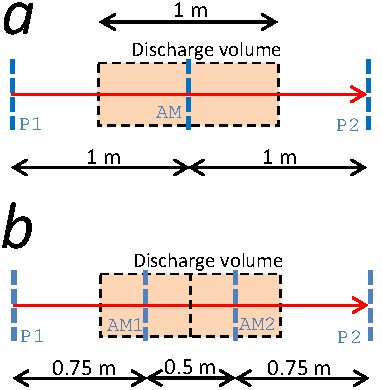
\includegraphics{images/layout}
\caption{Example of \texttt{layout} configuration for a long \texttt{optic} (in this case, an \textit{Active Medium}). a) The \textit{Active Medium} is represented by a single \texttt{optic}. b) The \textit{Active Medium} is split into two shorter sections.}\label{fig:layout}
\end{figure}
The corresponding \texttt{layout} configuration is:

\begin{verbatim}
#=========================
# long amplifier

- go: P1 >> 1 >> AM >> 1 >> P2
  times: 1
#=========================
\end{verbatim}

Alternatively, the active medium can be represented by two 0.5-meter sections, as shown in Fig.~\ref{fig:layout}b. The corresponding layout is:

\begin{verbatim}
#=========================
# long amplifier divided into two shorter sections

- go: P1 >> 0.75 >> AM1 >> 0.5 >> AM2 >> 0.75 >> P2
  times: 1
#=========================
\end{verbatim}

By splitting a long amplifier into shorter sections, the population dynamics within each amplifier section is modeled more accurately, leading to a more realistic representation of the active medium.


%%%%%%%%%%%%%
\subsection{Modeling of \texttt{Pulse} Propagation Between \texttt{Optics}}\label{propagation}

Consider free-space wave propagation between plane-parallel surfaces \(S'\) and \(S\), separated by distance \(z\), as illustrated in Fig.~\ref{fig:diffraction} for a system with cylindrical symmetry.
\begin{figure}[ht] 
 \centering
 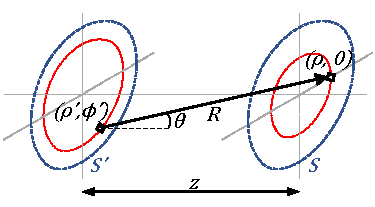
\includegraphics[width=10cm]{images/diffraction.pdf}
 \caption{Application of the Huygens-Fresnel principle to beam propagation from plane \(S'\) to plane \(S\) in a system with cylindrical symmetry.}
 \label{fig:diffraction}
\end{figure}
According to the Huygens-Fresnel principle, the field \(E\) at a point on plane \(S\) is defined as a superposition of secondary waves emitted from every point of plane \(S'\)~\cite{BornWolf:1999}. This can be expressed in the case of cylindrical symmetry as~\cite{Siegman:1986,PeatrossWare:2015}:
\begin{subequations} \label{eq:DI}
 \begin{align}
  &E(\rho) = -\frac{i}{\lambda} \int_{\rho'=0}^{\infty} E'(\rho') \int_{\phi'=0}^{2\pi} \frac{e^{ikR}}{R} K d\phi' \rho' d\rho' \label{eq:DI2a}\\
  &R = \sqrt{\rho^2 + \rho'^2 + z^2 - 2\rho\rho'\cos\phi'} \label{eq:DI2b}\\
  &K = \cos\theta = \frac{z}{R} \label{eq:DI2c}
 \end{align}
\end{subequations}
where \(\lambda\) is the wavelength, \(k = 2\pi / \lambda\) the wavenumber, and \(K\) the obliquity factor as it appears in Rayleigh-Sommerfeld diffraction theory.

Since the field on the output plane \(S\) does not depend on the angular coordinate \(\phi\), \(\phi = 0\) is chosen for the simplification of Eq.~\ref{eq:DI}.

Direct numerical integration of Eq.~\ref{eq:DI}, with \(O(N^3)\) complexity, is very time-consuming. Therefore, an approximation is usually employed to accelerate computations. The most well-known approximation is Fresnel diffraction, which assumes:
\begin{equation} \label{eq:FreA}
 \begin{split}
  &K \approx 1\\
  &R \approx
  \begin{cases}
   z & \text{(denominator)}\\
   z \left(1 + \frac{\rho^2 + \rho'^2 - 2\rho\rho'\cos\phi'}{2z^2}\right) & \text{(exponent)}
  \end{cases}
 \end{split}
\end{equation}
where "denominator" and "exponent" indicate the position of the \(R\) variable in Eq.~\ref{eq:DI2a}.

Substituting Eq.~\ref{eq:FreA} into Eq.~\ref{eq:DI2a} and using the formula
\begin{equation} \label{eq:formula}
 \int_{0}^{2\pi} e^{\pm i a \cos\phi}  d\phi = 2 \pi J_0(a)
\end{equation}
where \(J\) is the Bessel function, we obtain the expression for Fresnel diffraction with cylindrical symmetry:
\begin{equation} \label{eq:Fre}
 E(\rho) \approx -\frac{2 \pi i e^{ik\left(z+\frac{k\rho^2}{2z}\right)}}{\lambda z}
 \int_0^\infty E'(\rho') e^{i\frac{k\rho'^2}{2z}} J_0 \left(\frac{k\rho\rho'}{z}\right) \rho' d\rho'
\end{equation}

\textbf{\texttt{co2amp}} supports both Rayleigh-Sommerfeld (Eq.~\ref{eq:DI}) and Fresnel (Eq.~\ref{eq:Fre}) based propagation methods. Users can also choose to ignore the \texttt{pulse} evolution during free-space propagation.

Eqs.~\ref{eq:DI} and \ref{eq:Fre} assume monochromatic light, which is not the case for ultrashort pulses that possess a non-negligible bandwidth. Therefore, in \textbf{\texttt{co2amp}}, propagation is calculated in the frequency domain: Eqs.~\ref{eq:DI} or \ref{eq:Fre} are applied to the Fourier-transformed field at each node of the frequency calculation grid. Afterward, an inverse Fourier transform is used to return to the time domain.



%%%%%%%%%%%%%%%%%%%%%%%%%%%%%%%%%%%%%%%%%%%%%%%%%%%%%%%%%%%%%%%%%%%%%%%%%%%%%%%%%
\section{\texttt{Optic} Type A: \textit{Active Medium}}
The \textit{Active Medium} is the most complex type of \texttt{optic} that can be utilized in a \textbf{\texttt{co2amp}} project. Detailed models used for simulating molecular dynamics and \texttt{pulse} amplification are described in a dedicated Chapter~\ref{chapter:models}.

A configuration file for an \texttt{optic} of type A must include specifications of the gas mixture, pumping mechanism, and laser transitions considered in the simulations. An example of such a configuration file is provided below:

\begin{verbatim}
#=========================
# AM1.yml from 'examples/ATF 5 TW/ATF 3 final amplifier.co2' project

# Semi-diameter of the limiting aperture, m
semiDia: 45e-3

# Length of active medium, m
L: 0.57

# Gas mixture (bar)
p_CO2: 0.50
p_N2:  0.25
p_He:  7.50
O18:   0.472
C13:   0
T0:    300

# Bands included in calculations
band_reg: true
band_seq: true
band_hot: true

# Pumping
pumping: discharge
# Discharge volume, m^3
Vd: 0.0085
# Inter-electrode distance, m
D:  0.085
# Discharge profile
discharge: |
    0.00E+00 0.00000E+00 5.80000E+05
    1.00E-08 1.97186E+03 5.66356E+05
    2.00E-08 3.81445E+03 5.53030E+05
    3.00E-08 5.53410E+03 5.40019E+05
    4.00E-08 7.13691E+03 5.27312E+05
    ...
#=========================
\end{verbatim}

The composition of the active medium, including isotopic enrichment of carbon dioxide, and the initial temperature are specified under the "Gas mixture (bar)" section.

For discharge pumping, the geometry of the discharge and its temporal profile are required. In the case of optical pumping, the wavelength, absorption cross-section, and the temporal profile of the pumping pulse must be provided.

The 'optic~A~(discharge~pumped~CO2~amplifier).yml' and 'optic~A~(optically~pumped~CO2~amplifier).yml' template files contain detailed information on the configuration file format and can be referred to for further guidance.


%%%%%%%%%%%%%%%%%%%%%%%%%%%%%%%%%%%%%%%%%%%%%%%%%%%%%%%%%%%%%%%%%%%%%%%%%%%%%%%%%
\section{\texttt{Optic} Type P: \textit{Probe}}
A \textit{Probe} is a passive type of \texttt{optic}. It does not alter the field that fits within its semi-diameter. This can be expressed mathematically as:

\begin{equation}
E(t,\rho) = E'(t,\rho)
\end{equation}
where \( E'(t,\rho) \) and \( E(t,\rho) \) represent the field before and after passing through an \texttt{optic}, respectively.

However, a \textit{Probe} \texttt{optic} can serve as a limiting aperture, exhibiting zero transmittance for \( \rho > \text{semiDia} \). The sole configuration parameter for an \texttt{optic} of type P is its semi-diameter. An example of a configuration file for a \textit{Probe} with a 25 mm semi-diameter is shown below:

\begin{verbatim}
#=========================
# probe

semiDia: 25e-3
#=========================
\end{verbatim}


%%%%%%%%%%%%%%%%%%%%%%%%%%%%%%%%%%%%%%%%%%%%%%%%%%%%%%%%%%%%%%%%%%%%%%%%%%%%%%%%%
\section{\texttt{Optic} Type F: \textit{Spatial Filter}}
A \textit{Spatial Filter} applies a specified coordinate-dependent transmittance function to a \texttt{pulse}:

\begin{equation}
E(t,\rho) = E'(t,\rho) \sqrt{\mathcal{T}(\rho)}
\end{equation}
where \( \mathcal{T}(\rho) \) is the transmittance function, as defined in the configuration file.

An example configuration for a \textit{Spatial Filter} is shown below:

\begin{verbatim}
#=========================
# spatial filter

semiDia: 25e-3

filter: SIN
R: 10e-3
w: 10e-3
#=========================
\end{verbatim}

For more details and configuration options, refer to the 'optic~F~(spatial~filter).yml' template file.


%%%%%%%%%%%%%%%%%%%%%%%%%%%%%%%%%%%%%%%%%%%%%%%%%%%%%%%%%%%%%%%%%%%%%%%%%%%%%%%%%
\section{\texttt{Optic} Type S: \textit{Spectral Filter}}
A \textit{Spectral Filter} applies a specified frequency-dependent transmittance function to a \texttt{pulse}:

\begin{equation}
 \begin{aligned}
  &\widehat{E}'(\nu,\rho) = \mathcal{F}(E'(t,\rho))\\
  &\widehat{E}(\nu,\rho) = \widehat{E}'(\nu,\rho) \sqrt{\mathcal{T}(\nu)}\\
  &E(t,\rho) = \mathcal{F}^{-1}(\widehat{E}(\nu,\rho))
 \end{aligned}
\end{equation}
where \( \mathcal{F} \) and \( \mathcal{F}^{-1} \) denote the Fourier transform and the inverse Fourier transform, respectively, \( \nu \) is the frequency, and \( \mathcal{T}(\nu) \) is the transmittance function as defined in the configuration file.

An example configuration for a \textit{Spectral Filter} is provided below:

\begin{verbatim}
#=========================
# spectral filter

semiDia: 25e-3

filter: FREEFORM
form: |
    32.0e12 1.0
    32.1e12 0.9
    32.2e12 0.7
    32.3e12 0.5
    32.4e12 0.3
    32.5e12 0.0
    32.6e12 0.3
    32.7e12 0.5
    32.8e12 0.7
    32.9e12 0.9
    33.0e12 1.0
#=========================
\end{verbatim}

For further details and configuration options, refer to the 'optic~S~(spectral~filter).yml' template file.



%%%%%%%%%%%%%%%%%%%%%%%%%%%%%%%%%%%%%%%%%%%%%%%%%%%%%%%%%%%%%%%%%%%%%%%%%%%%%%%%%
\section{\texttt{Optic} Type L: \textit{Lens}}
A \textit{Lens} functions as a standard optical lens within the system:

\begin{equation}
 \begin{aligned}
  &\widehat{E}'(\nu,\rho) = \mathcal{F}(E'(t,\rho))\\
  &\widehat{E}(\nu,\rho) = \widehat{E}'(\nu,\rho) \exp\left( -\frac{i k \rho^2}{2 F} \right)\\
  &E(t,\rho) = \mathcal{F}^{-1}(\widehat{E}(\nu,\rho))
 \end{aligned}
\end{equation}
where \( k = \frac{2\pi\nu}{c} \) is the wave number (\( c \) is the speed of light) and \( F \) is the focal length of the lens.

The calculation is performed in the frequency domain to ensure that the effective focal length remains consistent across all frequencies in the pulse spectrum.

An example configuration for a lens with a 1-meter focal length is shown below:

\begin{verbatim}
#=========================
# lens (F = 1 m)

semiDia: 25e-3

F: 1.0
#=========================
\end{verbatim}


%%%%%%%%%%%%%%%%%%%%%%%%%%%%%%%%%%%%%%%%%%%%%%%%%%%%%%%%%%%%%%%%%%%%%%%%%%%%%%%%%
\section{\texttt{Optic} Type M: \textit{Material}}

In cases of oblique incidence, the effective intensity \(I_{\text{eff}}\) is reduced and the propagation distance in the material (effective thickness) \(\Theta_{\text{eff}}\) is automatically adjusted based on the incidence angle \(\theta_i\) and the refractive index \(n\):

\begin{equation}
 \begin{aligned}
   &\theta_r = \arcsin\left(\frac{\sin\theta_i}{n_0}\right)\\
   &I_{\text{eff}} = I \frac{\cos\theta_i}{\cos\theta_r}\\
   &\Theta_{\text{eff}} = \frac{\Theta}{\cos\theta_r} 
 \end{aligned}
\end{equation}
where \(I\) and \(\Theta\) are the intensity before the \texttt{optic} and the actual thickness of the material, respectively, and \(\theta_r\) is the refraction angle.

\subsubsection{Linear Dispersion and Absorption}
\begin{equation}
 \begin{aligned}
  &\widehat{E}'(\nu,\rho) = \mathcal{F}(E'(t,\rho))\\
  &\widehat{E}(\nu,\rho) = \widehat{E}'(\nu,\rho) \exp (2 \pi i \Delta \nu) \sqrt{\exp(-\alpha_0 \Theta_{\text{eff}})}\\
  &E(t,\rho) = \mathcal{F}^{-1}(\widehat{E}(\nu,\rho))
 \end{aligned}
\end{equation}
where \(\Delta \nu\) is defined as:
\begin{equation}\label{eq:Delta_nu_disp}
 \Delta \nu = \int_0^{\nu} (\nu'-\nu_c) \frac{dt}{d\nu'} d\nu',
\end{equation}
\begin{equation}
 \frac{dt}{d\nu'} = \frac{\Theta_{\text{eff}}}{c} \frac{dn_{g}}{d\nu'},
\end{equation}
with \(c\) as the speed of light, \(n_{g}\) as the group index of refraction, and \(\nu_c\) as the central frequency. The dispersion formulas used for calculating \(n_{g}\) are given in Appendix~\ref{appendix:optical_constants}.

\subsubsection{Nonlinear Interaction}
\begin{equation}
 \begin{aligned}
  &E(t,\rho) = E'(t,\rho) \exp\left(2\pi i \nu_c \frac{\Theta_{\text{eff}}}{c} n_2 I_{\text{eff}}(t,\rho)\right)\\
  &I_{\text{eff}}(t,\rho) = 2 h \nu_c (E'(t,\rho))^2 \frac{\cos\theta_i} {\cos\theta_r}
 \end{aligned}
\end{equation}
where \(n_2\) is the nonlinear refractive index, \(h\) is Planck's constant, and \(I(t,r)\) is the field intensity. Numerical values of \(n_2\) used in the program are given in Appendix~\ref{appendix:optical_constants}.

Configuration example for a \textit{Material} \texttt{optic}:

\begin{verbatim}
#=========================
# material

semiDia: 25e-3

material:  NaCl
thickness: 100e-3
tilt: 0
slices: 10
#=========================
\end{verbatim}

Currently supported materials include AgBr, AgCl, \ce{BaF2}, CdTe, CsI, GaAs, Ge, IRG22 (AMTIR1), IRG24, IRG25, KBr, KCl, KRS5, NaCl, NaF, Si, \ce{SiO2}, ZnS, ZnSe, and air. An arbitrary \(n_2\) can be specified in the configuration file, with a predefined value used otherwise (see Appendix~\ref{appendix:optical_constants}). To enhance accuracy, the \textit{Material} \texttt{optic} can be divided into several layers. A split-step method is employed for calculating linear and nonlinear interactions with a layer: first, a nonlinear interaction with a half-layer is calculated, followed by a full-layer linear interaction, and then a half-layer nonlinear interaction again.



%%%%%%%%%%%%%%%%%%%%%%%%%%%%%%%%%%%%%%%%%%%%%%%%%%%%%%%%%%%%%%%%%%%%%%%%%%%%%%%%%
\section{\texttt{Optic} Type C: \textit{Chirper}}
A \textit{Chirper} introduces a chirp to a pulse and is typically used to model a stretcher or compressor.

\begin{equation}
\begin{aligned}
&\widehat{E}'(\nu,\rho) = \mathcal{F}(E'(t,\rho))\\
&\widehat{E}(\nu,\rho) = \widehat{E}'(\nu,\rho) \exp(2 \pi i \Delta\nu)\\
&E(t,\rho) = \mathcal{F}^{-1}(\widehat{E}(\nu,\rho))
\end{aligned}
\end{equation}
where 
\begin{equation}\label{eq:Delta_nu_chirp}
 \Delta \nu = \int_0^{\nu} (\nu'-\nu_c) \frac{dt}{d\nu'} d\nu',
\end{equation}
\(\nu_c\) is the central frequency, and \(\frac{d\nu}{dt}\) is the chirpyness.

In the case of linear chirp, the chirpyness is constant, and Eq.~\ref{eq:Delta_nu_chirp} simplifies to:

\begin{equation}
\begin{aligned}
&\Delta \nu = \int_0^{\nu} \frac{\nu'-\nu_c}{\mathcal{C}} d\nu' = \frac{(\nu-\nu_c)^2}{2\mathcal{C}}\\
&\mathcal{C} = \frac{d\nu}{dt}
\end{aligned}
\end{equation}

An example configuration for a \textit{Chirper} with linear chirp is shown below:

\begin{verbatim}
#=========================
# stretcher (positive chirpyness => red chirp)

semiDia: 25e-3

chirp: LINEAR
c: 3.5e21
#=========================
\end{verbatim}

Currently, only linear chirp is supported in the program.


%%%%%%%%%%%%%%%%%%%%%%%%%%%%%%%%%%%%%%%%%%%%%%%%%%%%%%%%%%%%%%%%%%%%%%%%%%%%%%%%%
%%%%%%%%%%%%%%%%%%%%%%%%%%%%%%%%%%%%%%%%%%%%%%%%%%%%%%%%%%%%%%%%%%%%%%%%%%%%%%%%%
%%%%%%%%%%%%%%%%%%%%%%%%%%%%%%%%%%%%%%%%%%%%%%%%%%%%%%%%%%%%%%%%%%%%%%%%%%%%%%%%%
\chapter{Modelling of processes in \texorpdfstring{\ce{CO2}}{CO2} amplifiers}\label{chapter:models}

\section{Molecular dynamics}
Simulations of active medium pumping by electric discharge and vibrational relaxation are done following Karlov and Konev  \cite{Karlov-1978}.

\subsection{Pumping by electric discharge}
Pumping is described by the Boltzmann equation in the following form \cite{Holstein-1946,Nighan-1970}:

\begin{align}\label{eq:boltzmann}
&- \frac{1}{3} \left(\frac{\mathcal{E}}{\mathcal{N}}\right)^2 \frac{d}{du} \left[u \left( \sum\limits_j y_j Q_{mj}(u) \right)^{-1}\frac{df(u)}{du} \right] \quad = \nonumber \\
&\qquad \qquad 1.09 \times 10^{ - 3}\frac{d}{du}\left[ u^2 f(u)\sum\limits_j \frac{y_j}{M_j} Q_{mj}(u) \right]
\quad  + \quad \sum\limits_{j = 1,2} {y_j}{C_j} \frac{d}{du}(uf(u))
\quad  + \quad 6B y_2 \frac{d}{du}\left(uQ(u)f \right)\nonumber \\
&\qquad \qquad +\quad\sum\limits_j y_j \sum\limits_k (u + u_{jk})Q_{jk} (u + u_{jk})f(u + u_{jk}) \quad  - \quad uf(u)\sum\limits_j y_j \sum\limits_k Q_{jk}(u)
\end{align}
where the left part describes the energy of electrons in the electric field, the first component of the sum of the right part represents energy transfer via elastic collisions between electrons and molecules, the second and third components describe collisions with molecular rotation excitation, and the two last components relate to inelastic collisions with transfer of the energy $u_{jk}$ into vibrational and electronic excitations and ionization.

Electron energy $u$ is expressed in eV;

Ratio of the electric field to the full molecular density, $\mathcal{E}/\mathcal{N}$, is expressed in units of $10^{-16}$~V·cm$^2$;

$y_j$ are the relative molecule concentrations ($j=1$ corresponds to \ce{CO2}, $j=2$ to N$_2$ and $j=3$ to He);

$M_1=44$, $M_2=28$, $M_3=4$ are the molar masses;

$C_1 = 8.2 \times 10^{-4}$ eV·Å$^2$ \cite{Hake-1967};

$C_2 = 5.06 \times 10^{-4}$ eV·Å$^2$ \cite{Frost-1962};

$B = 2.5 \times 10^{-4}$ eV is the N$_2$ rotational constant.

Numerical values of the cross-sections $Q$ and the transferred energies $u_{jk}$ are summarized in Appendix \ref{appendix:crossections} 

Equation \ref{eq:boltzmann} is solved numerically using the tridiagonal matrix algorithm. Distribution function $f(u)$ is then used in the following calculations.

The rate constant $\omega_{jk}$, and the electron drift speeds $v_d$ are defined as:

\begin{equation}\label{eq:omega_jk}
\omega _{jk}\left[\frac{\rm{cm}^3}{\text{s}} \right] = 5.93 \times 10^{-9}\int\limits_0^\infty u Q_{jk}(u)f(u)du
\end{equation}
     
\begin{equation}\label{eq:v_d}
v_d \left[ \frac{\text{cm}}{\text{s}} \right] =  - 5.93 \times 10^7 \left( \frac{1}{3}\frac{\mathcal{E}}{\mathcal{N}} \right)\frac{df(u)}{du} \int\limits_0^\infty u \left( \sum\limits_j y_j Q_{mj}(u) \right)^{-1} du
\end{equation}

The fraction of electron energy transmitted via inelastic processes is defined as

\begin{equation}\label{eq:z_jk}
z_{jk} = 10^{16} \frac{y_j u_{jk} \omega _{jk}} {\left( \frac{\mathcal{E}}{\mathcal{N}} \right) v_d}   
\end{equation}

The fraction of electron energy transmitted to translations and rotations are the following:

\begin{equation}\label{eq:z_t}
z_t = 5.93 \times 10^7 \frac{1.09 \times 10^{-3} \int\limits_0^\infty u^2 \left( \sum\limits_j \frac{y_j}{M_j} Q_{mj}(u) \right)f(u)du} {\left( \frac{\mathcal{E}}{\mathcal{N}} \right) v_d}
\end{equation}

\begin{equation}\label{eq:z_r}
z_r = 5.93 \times 10^7 \frac{\sum\limits_{j=1,2} y_j C_j \int\limits_0^\infty uf(u)du + 6 y_2 B \int\limits_0^\infty u Q(u) f(u) du} {\left( \frac{\mathcal{E}}{\mathcal{N}} \right) v_d} 
\end{equation}

Finally, the distribution of the excitation energy is calculated using the following expressions:

$q_2 = \sum\limits_{k=1}^6 z_{1k}$ - fraction of energy transferred to \ce{CO2} symmetric stretch ($\nu_1$) and bending ($\nu_2$) modes;

$q_3 = z_{17}$ - fraction of energy transferred to \ce{CO2} asymmetric stretch mode ($\nu_3$);

$q_4 = \sum\limits_{k=1}^8 z_{2k}$ - fraction of energy transferred to \ce{N2} vibrations;

$q_T = z_t + z_r$ - fraction of energy transferred to translation and rotation;

$q_{ei} = \sum\limits_{k=9}^{15} z_{2k}  + \sum\limits_{k=8}^{10} z_{1k}$ - fraction of energy spent on excitation of electronic levels and ionization.



\subsection{Pumping and vibrational relaxation dynamics}
A 3-temperature model is used for describing the vibrational dynamics of the active medium of \ce{CO2} amplifiers. In this model, the following temperatures are used to describe the distribution of the energy between molecular vibrations:

$T_2$ – vibrational temperature of $\nu_1$ and $\nu_2$ vibrations of \ce{CO2};

$T_3$ – vibrational temperature of the $\nu_3$ vibration of \ce{CO2};

$T_4$ – vibrational temperature of \ce{N2}.

Vibrational temperatures are related to the average numbers of quanta $e_x$ in the corresponding vibrations as follows:

\begin{equation}\label{eq:e}
\begin{aligned}
&{e_2} = \frac{2}{\exp(960/{T_2})-1}\\
&{e_3} = \frac{1}{\exp(3380/{T_3})-1}\\
&{e_4} = \frac{1}{\exp(3350/{T_4})-1} 
\end{aligned}
\end{equation}
"2" in the first equation is due to 2-fold degeneracy of the energy levels of the bend vibration.

The dynamics of pumping/relaxation is described by the following equations

\begin{equation}\label{eq:dedt}
\begin{aligned}
&\frac{d e_4}{dt} = p_{e4} - r_a (e_4 - e_3)\\
&\frac{d e_3}{dt} = p_{e3} + r_c(e_4 - e_3) - r_3 f_3\\
&\frac{d e_2}{dt} = f_2 \left( p_{e2} + 3 r_3 f_3 - r_2 (e_2 - e_{2T}) \right)
\end{aligned}
\end{equation}
where
\begin{equation}\label{eq:dedt_rates}
\begin{aligned}
&p_{e4} = 0.8\times 10^{-3} \frac{q_4}{n y_2} W(t);\quad p_{e3} = 0.8\times 10^{-3}\frac{q_3}{n y_1} W(t);\quad p_{e2} = 2.8\times 10^{-3}\frac{q_2}{n y_1} W(t);\\
&f_2 = \frac{2(1+e_2)^2}{2+6e_2+3{e_2}^2};\quad f_3 = e_3(1+e_2/2)^3 - (1+e_3)(e_2/2)^3 \exp(- 500/T);\\
&r_a = kny_1;\quad r_c = kny_2;\quad r_2 = k_2n;\quad r_3 = k_3n;\\
&k_2 = \sum\limits_{i=1}^3 y_i k_{2i};\quad k_3 = \sum\limits_{i=1}^3 y_i k_{3i};\\
&n = 273 \frac{p[\text{bar}]}{T_0[\text{K}]};\\
&e_{2T} = \frac{2}{\exp(960/T)-1}
\end{aligned}
\end{equation}
where $W(t)$ is the discharge power density measured in {kW/cm$^3$} , $p_e$ is measured in \si{\micro\second^{-1}}, and the constants $k$ are calculated using the following expressions \cite{Biryukov-1974,Taylor-1969}:

\begin{equation}
\begin{aligned}
&k = 240 / T^{1/2};\\
&k_{31} = A(t)\exp(4.138 + 7.945x - 631.24x^2 + 2239x^3);\\
&k_{32} = A(t)\exp(-1.863 + 213.3x - 2796.2x^2 + 9001.9x^3);\\
&k_{33} = A(t)\exp(-3.276 + 291.4x - 3831.8x^2 + 12688x^3);\\
&k_{21} = 1.16 \times 10^3 \exp(-59.3x);\\
&k_{22} = 8.55 \times 10^2 \exp(-69x);\\
&k_{23} = 1.3 \times 10^3 \exp(-40.6x)
\end{aligned}
\end{equation}
where $x=T^{-1/3}$, $A(t)=(T/273)(1+e_{2T}/2)^{-3}$, and temperature $T$ is expressed in K.

Finally, the dynamics of the gas temperature is described by the following equation:

\begin{equation}\label{eq:dTdt}
\frac{dT}{dt} = \frac{y_1}{C_V}(500r_3f_3 + 960r_2(e_2-e_{2T})) + 2.7\frac{W(t)q_T}{nC_V},
\end{equation}
where $C_V = 2.5(y_1+y_2) + 1.5y_3$.


\subsection{Optical pumping}
In the case of optical pumping population dynamics is modelled with equations \ref{eq:e}--\ref{eq:dTdt} with the exception of the expressions for excitation rates in Eq.~\ref{eq:dedt_rates} that are replaced by

\begin{equation}\label{eq:dedt_rates_optical}
\begin{aligned}
&p_{e4} = 0;\\
&p_{e3} = \Phi \sigma;\\
&p_{e2} = \left\{
  \begin{array}{>{\displaystyle}l>{\displaystyle}l}
  0             & direct~excitation~of~(00^01)~at~\sim4.3~{\mu}m\\
  2 \Phi \sigma & excitation~via~(10^01, 02^01)~at~\sim2.8~{\mu}m\\
  4 \Phi \sigma & excitation~via~(20^01, 12^01, 04^01)~at~\sim2.0~{\mu}m
  \end{array}
  \right.
\end{aligned}
\end{equation}
where $\Phi$ is the flux of the pumping photons (number of photons per $\text{m}^2$ per second), and $\sigma$ is the absorption cross-section. Equations \ref{eq:dedt_rates_optical} imply that each pumping photon delivers one quantum of energy to the upper laser level, and zero, two or four quanta to the lower level, depending on the pumping transition.


\section{Amplification}


\subsection{Isotopologues of \ce{CO2} and their nomenclature}

The \textbf{\texttt{co2amp}} model includes six isotopologues of \ce{CO2} with different combinations of stable isotopes of carbon (\ce{^{12}C} and \ce{^{13}C}) and oxygen (\ce{^{16}O} and \ce{^{18}O}). A commonly used three-digit notation designates the isotopologues of carbon dioxide, where each digit represents the isotope of an atom in the molecule in the order oxygen–carbon–oxygen, corresponding to the last digit of the isotope's mass number. In this notation, the digits \textit{2} and \textit{3} represent \ce{^{12}C} and \ce{^{13}C}, respectively, while the digits \textit{6} and \textit{8} represent \ce{^{16}O} and \ce{^{18}O}, respectively. Thus, \textit{626}, for instance, denotes a \ce{CO2} molecule with the natural isotopic composition \ce{^{16}O}-\ce{^{12}C}-\ce{^{16}O}, and \textit{638} stands for the \ce{^{16}O}-\ce{^{13}C}-\ce{^{18}O} isotopologue.




\subsection{Vibrational levels of \ce{CO2} molecule}

\subsubsection{Laser transitions}

Laser transitions in \ce{CO2} amplifiers occur between the rotational sub-levels of vibrational levels in the electronic ground state of the molecule. The primary laser transitions (''Regular bands'') are between the first excited state of the antisymmetric stretching vibration and one of the combination vibrations involving the first excited state of the symmetric stretching and the second excited state of the bending vibration. However, transitions between higher energy levels are also possible, potentially contributing to the overall gain of the amplifier. Multiple vibrational energy levels are thus included in the \textbf{\texttt{co2amp}} amplification model. Figure~\ref{fig:laser-transitions} shows some of the laser transitions included in the \textbf{\texttt{co2amp}} amplification model and the vibrational levels involved in these transitions.

\begin{figure}[ht]
\centering
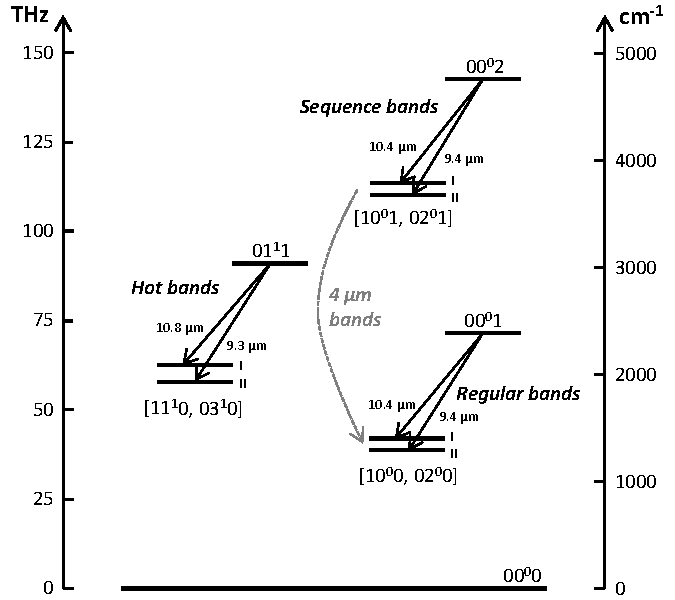
\includegraphics[width=120mm]{images/laser-transitions}
\caption{Vibrational transitions included in the amplification model. Wavelengths are given for natural \ce{CO2} isotopologue (\textit{626}).}\label{fig:laser-transitions}
\end{figure}

Other vibrational levels contributing to the population dynamics of the laser levels are not shown in the figure but are included in the model as described in the following text. Additionally, the code includes experimental support for modeling laser transitions at approximately \SI{4}{\micro\meter} between the group of levels at the end of the sequence bands and the group of levels including the lower levels of the regular bands. Below, we describe the basics of the involved molecular spectroscopy, followed by the description of the model of the population dynamics and stimulated emission.



\subsubsection{Vibrational level nomenclature}

A standard scheme of vibrational level nomenclature uses the $\nu_1\,\nu_2^{l[e/f]}\,\nu_3$ notation, where $\nu_1$, $\nu_2$, and $\nu_3$ are the numbers of quanta in the symmetric stretch, bending, and antisymmetric stretch vibrational modes, respectively, and $l$ is the vibrational angular momentum quantum number of the doubly degenerate bending vibration. States with $l \neq 0$ are further split into two sub-levels due to the two possible symmetries associated with the bending vibration. A letter $e$ or $f$ is added to the notation after the value of $l$ to differentiate between these sub-levels.

In the \ce{CO_2} molecule, a strong Fermi coupling exists between the $\nu_1$ and $\nu_2$ vibrations, resulting in mixed states that cannot be directly attributed to a single set of vibrational quantum numbers. We refer to these levels by listing the contributing states in square brackets and adding a Roman numeral subscript indicating a sub-level number. For instance, the lower laser level of the \SI{9.4}{\micro\meter} regular band is denoted as $[1\,0^{0}0,\,0\,2^{0}0]_{\mathrm{II}}$.

In the HITRAN database, the symmetry of the bending vibration ($e$ or $f$) is associated with the rotational levels rather than with the vibrational ones, as in the \textbf{\texttt{co2amp}} model. Associating the symmetry with the vibrational state makes modeling the energy distribution between ro-vibrational sub-levels more straightforward and transparent. Also, the letter $e$ is associated with the $l = 0$ levels in HITRAN for database consistency.

Furthermore, in HITRAN, the mixed states are labeled by one of the contributing states followed by a sub-level number. The $[1\,0^{0}0,\,0\,2^{0}0]_{\mathrm{II}}$ level, for example, is denoted as $1\,0^{0}0\,(2)$ (or $1\,0\,0\,0\,2$ in the raw \texttt{.par} files). The letter $e$ is then added to the rotational level labels (e.g., ''P 20e'').




\subsubsection{Vibrational levels included in the \textbf{\texttt{co2amp}} model}

Table \ref{tab:levels} lists the vibrational levels included in the model.

\begin{table}[h!]\label{tab:levels}
\centering
\caption{Vibrational Levels}
\begin{tabular}{c c c c p{8cm}}
\hline
\textbf{\#} & \textbf{Level} & \textbf{Parity} & \textbf{Weight} & \textbf{Description} \\
\hline
\noalign{\vspace{1.5ex}}
\multicolumn{5}{c}{\boldmath{$0\,0\,1$}} \\
[1.5ex]
0  & $0\,0^{0}1$  & $u$ & 1   & Upper level of regular bands \\
[1.5ex]
\multicolumn{5}{c}{\boldmath{$1\,0\,0 + 0\,2\,0$}} \\
[1.5ex]
1  & $[1\,0^{0}0,\,0\,2^{0}0]_{I}$  & $g$ & 1/3 & 1, 2: lower levels of regular bands \\
2  & $[1\,0^{0}0,\,0\,2^{0}0]_{II}$  & $g$ & 1/3 & 1, 2, 3, 4: lower levels of 4\,µm bands \\
3  & $0\,2^{2e}0$  & $g$ & 1/6 & \\
4  & $0\,2^{2f}0$  & $g$ & 1/6 & \\
[1.5ex]
\multicolumn{5}{c}{\boldmath{$0\,1\,1$}} \\
[1.5ex]
5  & $0\,1^{1e}1$  & $u$ & 1/2 & Upper levels of hot bands \\
6  & $0\,1^{1f}1$  & $u$ & 1/2 & \\
[1.5ex]
\multicolumn{5}{c}{\boldmath{$1\,1\,0 + 0\,3\,0$}} \\
[1.5ex]
7  & $[1\,1^{1e}0,\,0\,3^{1e}0]_{I}$  & $u$ & 3/16 & 7, 8, 9, 10: lower levels of hot bands \\
8  & $[1\,1^{1e}0,\,0\,3^{1e}0]_{II}$  & $u$ & 3/16 & 11, 12: not currently included in the  \\
9  & $[1\,1^{1f}0,\,0\,3^{1f}0]_{I}$  & $u$ & 3/16 & amplification model \\
10 & $[1\,1^{1f}0,\,0\,3^{1f}0]_{II}$  & $u$ & 3/16 & \\
11 & $0\,3^{3e}0$  & $u$ & 1/8 & \\
12 & $0\,3^{3f}0$  & $u$ & 1/8 & \\
[1.5ex]
\multicolumn{5}{c}{\boldmath{$0\,0\,2$}} \\
[1.5ex]
13 & $0\,0^{0}2$  & $g$ & $1$   & Upper level of sequence bands \\
[1.5ex]
\multicolumn{5}{c}{\boldmath{$1\,0\,1 + 0\,2\,1$}} \\
[1.5ex]
14 & $[1\,0^{0}1,\,0\,2^{0}1]_{I}$  & $u$ & 1/3 & 14, 15: lower levels of sequence bands \\
15 & $[1\,0^{0}1,\,0\,2^{0}1]_{II}$  & $u$ & 1/3 & 14, 15, 16, 17: upper levels of 4\,µm bands \\
16 & $0\,2^{2e}1$  & $u$ & 1/6 & \\
17 & $0\,2^{2f}1$  & $u$ & 1/6 & \\
\hline
\end{tabular}
\end{table}




The levels in the table are grouped to include sub-levels arising from angular momentum splitting and Fermi coupling between the $\nu_1$ and $\nu_2$ vibrations.


\subsubsection{Statistical weights of vibrational levels}

We assume a simple statistical distribution of the population among the levels in each group to assign a weight coefficient to each level. To demonstrate the procedure for calculating the weights, let's consider the group including levels \#1, \#2, \#3, and \#4.

We start from the normal mode populations; there are two modes involved:

- The mode $1\,0\,0$ contains half of the population (weight coefficient $\frac{1}{2}$) and has no splitting due to angular momentum, as the degenerate vibration $\nu_2$ is not involved. The only sub-level is thus $1\,0^{0}0$.

- The mode $0\,2\,0$ contains the other half of the population (weight coefficient $\frac{1}{2}$) and is split due to angular momentum into three sub-levels: $0\,2^{0}0$, $0\,2^{2e}0$, and $0\,2^{2f}0$. Each sub-level of $0\,2\,0$ thus has a weight coefficient of $\frac{1}{6}$ (since $\frac{1}{2}$ divided equally among three sub-levels).

Since $1\,0^{0}0$ and $0\,2^{0}0$ are coupled through Fermi resonance, their populations are assumed to redistribute equally between the resultant mixed levels (levels \#1 and \#2). Therefore, the weight coefficient for each mixed level is calculated as:

\[
\frac{ \text{Weight from } 1\,0^{0}0 + \text{Weight from } 0\,2^{0}0 }{2} = \frac{ \frac{1}{2} + \frac{1}{6} }{2} = \frac{1}{3}.
\]

Thus, each mixed level (\#1 and \#2) receives a weight coefficient of $\frac{1}{3}$.

The sub-levels resulting from the angular momentum splitting of $0\,2\,0$, namely $0\,2^{2e}0$ (level \#3) and $0\,2^{2f}0$ (level \#4), retain their individual weight coefficients of $\frac{1}{6}$ each.

This approach ensures that the total population is conserved, and the weights assigned to each sub-level reflect the statistical distribution due to the coupling and splitting mechanisms.



\subsubsection{Populations of vibrational levels in thermal equilibrium}

In the approximation used in the \textbf{\texttt{co2amp}} model, the processes of pumping and vibrational relaxation are slow compared to the duration of the pulse. Thus, only the stimulated transitions contribute to the change of the populations of vibrational levels during the pulse.

In the fast time-frame associated with the pulse there is no equilibrium in the vibrational energy distribution, and a proper population dynamics rather than the temperature model must be used. Thus, during the amplification, population of each rotational-vibrational level is considered independently. After the pulse leaves the active medium, the energy distribution within each vibrational mode becomes normalized quickly, and can be described by the temperature model again.

An important simplification used in the model is the assumption that vibrational temperatures $T_2$ and $T_3$ are the same for all \ce{CO2} isotopologues. This assumption can be justified by the relatively small energy mismatch between vibrational levels of different isotopic species of the same molecule, and thus, fast inter-molecular V-V energy exchange. However, this assumption may not hold if the time-delay between two consecutive passes of a pulse through the amplifier is short compared to the relaxation times of intra-mode and inter-isotopic vibrational energy.


Initial populations of vibrational levels are calculated for each isotopologue and for each band by first calculating the total populations of the groups of levels defined in Table~\ref{tab:levels} using the following equations \ref{eq:Boltzman} and then applying the corresponding weights coefficients from the Table.

\begin{equation}\label{eq:Boltzman}
\begin{aligned}
N_{0\,0\,1}           &=   \frac{N}{\mathcal{Q}} \exp\left(\frac{-3380}{T_3}\right)\\
N_{1\,0\,0 + 0\,2\,0} &= 2 \frac{N}{\mathcal{Q}} \exp\left(\frac{-2\times 960}{T_2}\right)\\
N_{0\,1\,1}           &=   \frac{N}{\mathcal{Q}} \exp\left(\frac{-960}{T_2}\right) \exp\left(\frac{-3380}{T_3}\right)\\
N_{1\,1\,0 + 0\,3\,0} &= 2 \frac{N}{\mathcal{Q}} \exp\left(\frac{-3\times 960}{T_2}\right)\\
N_{0\,0\,2}           &=   \frac{N}{\mathcal{Q}} \exp\left(\frac{-2\times 3380}{T_3}\right)\\
N_{1\,0\,1 + 0\,2\,1} &= 2 \frac{N}{\mathcal{Q}} \exp\left(\frac{-2\times 960}{T_2}\right) \exp\left(\frac{-3380}{T_3}\right)
\end{aligned}
\end{equation}

where $N$ is the density of \ce{CO2} molecules, and $\mathcal{Q}$ the partition function \cite{Witteman-1987}:
\begin{equation}
\frac{1}{\mathcal{Q}} = \left(1-\exp\left(\frac{-1920}{T_2}\right)\right) \times \left(1-\exp\left(\frac{-3380}{T_3}\right)\right) \times \left(1-\exp\left(\frac{-960}{T_2}\right)\right)^2
\end{equation}






\subsection{Rotational sub-levels}

Rotational sub-level population in the rotational equilibrium is calculated as
\begin{equation}
N_{rot}^0(J) = z(J) \times s(J) \times N_{vib}.
\end{equation}

Here, \( N_{vib} \) is the total population density of the corresponding vibrational level.

$z(J)$ is the rotational Boltzmann distribution function defined by:

\begin{equation}\label{eq:z}
z(J) = \frac{hB}{kT}(2J+1)\exp \left(-\frac{hB}{kT}J(J+1)\right)
\end{equation}
where $B$ is the rotational constant, $h = 6.62606957\times 10^{-34}$~J·s and $k = 1.3806488\times 10^{-23}$~J/K

To determine the coefficient \( s(J) \), follow these steps:

\begin{itemize}
    \item If \( J < l \):
    \[s(J) = 0\]

    \item If \( J \geq l \):
    \begin{itemize}
        \item For symmetric isotopologues (\textit{626}, \textit{636}, \textit{828}, and \textit{838}):
        \begin{itemize}
            \item If parity = \(g\) and symmetry = \(e\) \quad or \quad  parity = \(u\) and symmetry = \(f\)
            \[
            s(J) = \begin{cases}
            2 & \text{for even } J \\
            0 & \text{for odd } J
            \end{cases}
            \]
            \item If parity = \(g\) and symmetry = \(f\) \quad or \quad  parity = \(u\) and symmetry = \(e\)
            \[
            s(J) = \begin{cases}
            0 & \text{for even } J \\
            2 & \text{for odd } J
            \end{cases}
            \]
        \end{itemize}

        \item For asymmetric isotopologues (\textit{628} and \textit{638}):
        \[s(J) = 1\]
    \end{itemize}
\end{itemize}

In the above:

\begin{itemize}
    \item \(l\) is the vibrational angular momentum. Rotational levels with \( J < l \) are not populated due to angular momentum coupling restrictions.
    \item The \textbf{parity} of the vibrational state is determined by the sum of quanta in the ungerade (\( u \)) vibrational modes (\( v_2 \) and \( v_3 \)):
    \[
    \text{parity} = \begin{cases}
    g & \text{if } v_2 + v_3 \text{ is even} \\
    u & \text{if } v_2 + v_3 \text{ is odd}
    \end{cases}
    \]
    \item The \textbf{symmetry} refers to the e/f symmetry labels of the rotational-vibrational levels, which are determined by the coupling of rotational angular momentum \( J \) and vibrational angular momentum \( l \). The e/f labels are adapted from the HITRAN database.
    \item For symmetric isotopologues, the statistical weight \( s(J) \) is 2 for allowed rotational levels due to nuclear spin statistical weights, and 0 for forbidden levels.
    \item For asymmetric isotopologues, there are no symmetry restrictions due to the lack of identical nuclei, so all rotational levels with \( J \geq l \) are equally populated, and \( s(J) = 1 \).
\end{itemize}



\subsection{Use of HITRAN data}

Data for the supported transitions are extracted from the HITRAN database \cite{Gordon-2022}. This includes transition frequencies $\nu_j$, Einstein coefficients $A_j$, and rotational quantum numbers of the upper and lower laser levels ($J_{U,j}$ and $J_{L,j}$, respectively). The rotational constants $B$ are determined by fitting the data with the following equation, where $V$, $B_U$, and $B_L$ are fitting parameters:

\begin{equation}\label{eq:frequencies}
\nu_j = V + B_U J_{U,j} (J_{U,j} + 1) - B_L J_{L,j} (J_{L,j} + 1).
\end{equation}

Here, $j$ indexes the transitions involved in the model. The fitting is performed separately for each vibrational band of each isotopologue, using only the ro-vibrational transitions $j$ belonging to that band. The values of $B$ are summarized in Appendix~\ref{appendix:molecular_constants}.



\subsection{Modeling the amplification}
Amplification is simulated in the fast time-frame moving with the pulse using the following equations that also take into account rotational relaxation \cite{Feldman-1973,Volkin-1979}:

\begin{equation}\label{eq:amplification}
\begin{aligned}
&\frac{\partial E}{\partial z} =  - \sum\limits_j {\rho _j},\\
&\frac{\partial \rho _j}{\partial t} + \left(2\pi i(\nu _c-\nu _{0j}) + \frac{1}{\tau_2} \right)\rho _j =  - \frac{\sigma _j n_j E}{2\tau_2},\\
&\frac{\partial n_j}{\partial t} + \frac{n_j-n_j^0}{\tau _R} = 4(\rho _j E^* + c.c.),
\end{aligned}
\end{equation}
where summation is done over all rotational-vibrational transitions of all \ce{CO2} isotopologues, and

$E$ - complex field envelope,

$\rho_j$ - polarization of the medium,

$z$ - linear coordinate along the direction of beam propagation,

$t$ - time,

$n_j$ - population inversion of the transition (difference of population densities of upper and lower levels),

$n_j^0$ - equilibrium population inversion of the transition,

$\nu _c$ - carrier frequency,

$\nu_{0j}$ - transition frequency in the line center,

$\sigma_j$ - transition cross-section in the line center,

$\tau_2$ - polarization dephasing time,

$\tau_R$ - rotational relaxation time.



The line-center cross-section is calculated using the expression \cite{Hilborn-2002}:

\begin{equation}\label{eq:sigma}
\sigma_j\ [\text{m}^2] = \frac{ (\lambda_j\ [\text{m}])^2\, A_j\ [\text{s}^{-1}] }{4} \times \frac{ \tau_2\ [\text{s}] }{ \pi }.
\end{equation}

Here, the first term represents the integrated cross-section of the rotational line, and the second term gives the maximum of the normalized Lorentzian profile of a line with a half-width at half-maximum (HWHM) of $\Delta \nu_{\text{HWHM}} = 1/(2\pi \tau_2)$.

Optical intensity $I$ is related to the field amplitude as follows:
\begin{equation}\label{eq:I}
I[\text{W/m}^2] = 2 h[\text{J·s}] \nu _c[\text{s}^{-1}] |E|^2
\end{equation}

Dephasing and relaxation times are defined by the following equations:
\begin{equation}\label{eq:relaxation}
\begin{aligned}
&\tau_2[\text{s}] = \frac{10^{- 6}}{\pi \times 7.61 \times 750 \times (P_{CO2}+0.733P_{N2}+0.64P_{He})}\\
&\tau _R[\text{s}] = \frac{10^{-7}}{750 \times (1.3P_{CO2}+1.2P_{N2}+0.6P_{He})}
\end{aligned}
\end{equation}
where pressure $P$ is measured in bars.


The change in population due to stimulated transitions is calculated for each vibrational level of each isotopologue using the last equation from Equations~\eqref{eq:amplification}:

\begin{equation}\label{eq:dNdt}
\begin{aligned}
\frac{d}{dt} N_U &= 2 \sum_{j} \left( \rho_J E^* + \text{c.c.} \right), \\
\frac{d}{dt} N_L &= -2 \sum_{j} \left( \rho_J E^* + \text{c.c.} \right),
\end{aligned}
\end{equation}

where the summation is over all rotational transitions originating from ($N_U$) or ending at ($N_L$) the corresponding vibrational level.

In the next step, we calculate the overall change in the $\nu_2$ and $\nu_3$ quanta, denoted as $\Delta N_{\nu_2}$ and $\Delta N_{\nu_3}$, respectively. This is done by summing the population changes of all levels for all isotopologues, multiplying each by the number of corresponding quanta in the given level. In this calculation, we consider each $\nu_1$ quantum as equivalent to two $\nu_2$ quanta, an approximation based on the assumption of equal $T_1$ and $T_2$ temperatures due to Fermi coupling.

The changes in the average quantum numbers in the vibrational modes due to stimulated transitions are calculated as follows:

\begin{equation}\label{eq:Deltae}
\begin{aligned}
\Delta e_3 &= \frac{\Delta N_{\nu_3}}{N}, \\
\Delta e_2 &= \frac{\Delta N_{\nu_2}}{N} \times \frac{e'_2}{2 e'_1 + e'_2},
\end{aligned}
\end{equation}

where the last factor in the second equation accounts for the equilibrium energy distribution between the coupled symmetric stretch ($\nu_1$) and bending ($\nu_2$) vibrations. Here, $e'_1$ and $e'_2$ are the equilibrium average quantum numbers given by:

\[
e'_1 = \frac{1}{\exp\left( \frac{1920}{T_2} \right) - 1}, \quad e'_2 = \frac{2}{\exp\left( \frac{960}{T_2} \right) - 1},
\]

and $T_2$ is the vibrational temperature before the propagation of the pulse.





New vibrational temperatures are then calculated with Eq.~\ref{eq:e}.


\begin{appendices}


\chapter{Cross-sections of excitation processes}
\label{appendix:crossections}

Effective cross-sections are expressed in Å; their numerical values in the nodes are given in the tables below (linear interpolation must be used for determining the values in intermediate points); the data and citations are reproduced from \cite{Karlov-1978}.


The following notation for cross-sections is used:

$Q_{m1}$ - Transport cross-section of \ce{CO2} \cite{Lowke-1973};

$Q_{m2}$ - Transport cross-section of \ce{N2} \cite{Frost-1962};

$Q_{m3}$ - Transport cross-section of He \cite{Lowke-1973};

$Q$ - Cross-section of resonant excitation of \ce{N2} rotation  \cite{Oksyuk-1966,Chandra-1973};

$Q_{11}$ - Cross-section of the process $(000)\rightarrow(01^10)$  \cite{Lowke-1973};

$Q_{12}$ - Cross-section of the process $(000)\rightarrow(100+020)$  \cite{Lowke-1973};

$Q_{13}...Q_{16}$ - Cross-sections of resonant processes around 3.8 eV  \cite{Lowke-1973};

$Q_{17}$ - Cross-section of the process $(000)\rightarrow(001)$  \cite{Lowke-1973};

$Q_{18}...Q_{1,10}$ - Cross-sections of electronic excitation and ionization of \ce{CO2}  \cite{Hake-1967};

$Q_{21}...Q_{28}$ - Cross-sections of the process \ce{N2}$(v=0)\rightarrow$\ce{N2}$(v=1...8)$ \cite{Phelps-1968,Schulz-1962,Engelhardt-1964};

$Q_{29}...Q_{2,15}$ - Cross-sections of electronic excitation and ionization of \ce{N2} \cite{Engelhardt-1964}. 

\begin{table}
\centering
\caption{Cross-sections and energies for discharge pumping}
\begin{tabular}{|c|c||c|c||c|c||c|c|}
\hline 
$u_i$ & $Q_{m1}$ & $u_i$ & $Q_{m2}$ & $u_i$ & $Q_{m3}$ & $u_i$ & $Q$ \\ 
\hline
0    & 140  & 0     & 1.4  & 0    & 5   & 0.0015 & 0    \\
0.04 & 84   & 0.001 & 1.4  & 0.01 & 5.4 & 0.05   & 0.1  \\
0.1  & 55   & 0.002 & 1.6  & 0.1  & 5.8 & 0.25   & 0.65 \\
0.3  & 21   & 0.008 & 2    & 0.2  & 6.2 & 0.5    & 1.15 \\
0.5  & 10.8 & 0.01  & 2.2  & 1    & 6.5 & 0.8    & 2    \\
0.6  & 9.4  & 0.04  & 4    & 2    & 6.1 & 1      & 2.65 \\
1    & 5.7  & 0.08  & 6    & 7    & 5   & 1.5    & 5.6  \\
1.7  & 5    & 0.1   & 6.5  & 10   & 4.1 & 1.8    & 7.5  \\
2    & 5.1  & 0.2   & 8.8  & 20   & 3   & 1.9    & 8.2  \\
2.5  & 6    & 0.3   & 9.8  &      &     & 2      & 8.6  \\
3    & 7.7  & 0.4   & 10   &      &     & 2.15   & 8.95 \\
4.1  & 9.4  & 1     & 10   &      &     & 2.43   & 9    \\
5    & 14.5 & 1.2   & 11   &      &     & 2.6    & 8.9  \\
7.4  & 10   & 1.4   & 12.5 &      &     & 2.75   & 8.4  \\
10   & 11.7 & 1.8   & 20   &      &     & 2.9    & 7.65 \\
20   & 16   & 2     & 25   &      &     & 3.25   & 6.2  \\
27   & 16.3 & 2.5   & 30   &      &     & 3.6    & 5.1  \\
50   & 13   & 3     & 26   &      &     & 4      & 4.5  \\
     &      & 4     & 15   &      &     & 4.5    & 4.16 \\
     &      & 5     & 12   &      &     & 5      & 3.97 \\
     &      & 7     & 10   &      &     & 5.5    & 3.93 \\
     &      & 10    & 10   &      &     & 7      & 4.17 \\
     &      & 14    & 11   &      &     & 9      & 4.46 \\
     &      & 18    & 12.2 &      &     & 11     & 4.42 \\
     &      & 20    & 12   &      &     & 15     & 3.94 \\
     &      & 30    & 10   &      &     & 22     & 3.15 \\
     &      & 100   & 10   &      &     & 25     & 3.05 \\
\hline
\end{tabular}
\end{table}

\begin{table}
\centering
\caption{Cross-sections and energies for discharge pumping - continued}
\begin{tabular}{|c|c||c|c||c|c||c|c||c|c|}
\hline 
$u_i$ & $Q_{11}$ & $u_i$ & $Q_{12}$ & $u_i$ & $Q_{13}$ & $u_i$ & $Q_{14}$ & $u_i$ & $Q_{15}$ \\
\hline 
0.083 & 0    & 0.167 & 0    & 0.252 & 0    & 2.37 & 0    & 2.37 & 0    \\
0.085 & 0.36 & 0.2   & 0.54 & 2.7   & 0.25 & 3    & 0.26 & 3    & 0.17 \\
0.09  & 1.04 & 0.25  & 0.82 & 3     & 0.4  & 3.5  & 0.52 & 3.65 & 0.33 \\
0.1   & 1.6  & 0.3   & 0.82 & 3.3   & 0.6  & 4    & 0.5  & 3.8  & 0.31 \\
0.12  & 1.84 & 0.5   & 0.68 & 3.6   & 0.65 & 4.5  & 0.22 & 4    & 0.21 \\
0.14  & 2.12 & 0.7   & 0.56 & 4.5   & 0.23 & 4.6  & 0.1  & 4.3  & 0.1  \\
0.16  & 2.16 & 1     & 0.47 & 4.6   & 0.1  & 5    & 0    & 5    & 0    \\
0.2   & 2.08 & 1.4   & 0.45 & 5     & 0    &      &      &      &      \\
0.3   & 1.76 & 2     & 0.55 &       &      &      &      &      &      \\
0.4   & 1.52 & 3     & 1.15 &       &      &      &      &      &      \\
0.5   & 1.28 & 3.9   & 1.83 &       &      &      &      &      &      \\
0.6   & 1.08 & 4.5   & 1.4  &       &      &      &      &      &      \\
0.8   & 0.8  & 5     & 0.4  &       &      &      &      &      &      \\
1     & 0.58 & 6     & 0.28 &       &      &      &      &      &      \\
1.2   & 0.48 & 10    & 0.2  &       &      &      &      &      &      \\
1.6   & 0.34 & 20    & 0.1  &       &      &      &      &      &      \\
1.8   & 0.35 &       &      &       &      &      &      &      &      \\
2     & 0.4  &       &      &       &      &      &      &      &      \\ 
2.5   & 0.64 &       &      &       &      &      &      &      &      \\ 
3     & 1.04 &       &      &       &      &      &      &      &      \\ 
3.7   & 1.4  &       &      &       &      &      &      &      &      \\ 
4     & 1.36 &       &      &       &      &      &      &      &      \\ 
4.2   & 1.2  &       &      &       &      &      &      &      &      \\ 
4.5   & 0.92 &       &      &       &      &      &      &      &      \\ 
5     & 0.53 &       &      &       &      &      &      &      &      \\ 
6     & 0.4  &       &      &       &      &      &      &      &      \\ 
8     & 0.36 &       &      &       &      &      &      &      &      \\ 
9     & 0.28 &       &      &       &      &      &      &      &      \\ 
10    & 0.16 &       &      &       &      &      &      &      &      \\ 
10.1  & 0    &       &      &       &      &      &      &      &      \\
\multicolumn{2}{|c||}{$u_{11}=0.083$ eV} &
\multicolumn{2}{c||}{$u_{12}=0.167$ eV} &
\multicolumn{2}{c||}{$u_{13}=0.252$ eV} &
\multicolumn{2}{c||}{$u_{14}=0.339$ eV} &
\multicolumn{2}{c|}{$u_{15}=0.422$ eV}\\
\hline
\hline 
$u_i$ & $Q_{16}$ & $u_i$ & $Q_{17}$ & $u_i$ & $Q_{18}$ & $u_i$ & $Q_{19}$ & $u_i$ & $Q_{1,10}$ \\                                                                             
\hline
2.5  & 0     & 0.29 & 0    & 7    & 0     & 10.5 & 0    & 13.8 & 0    \\
3    & 0.19  & 0.3  & 0.44 & 8    & 0.5   & 11.5 & 0.56 & 15   & 0.1  \\
3.6  & 0.245 & 0.35 & 0.65 & 8.4  & 0.6   & 14   & 0.8  & 16   & 0.13 \\
4    & 0.21  & 0.4  & 0.73 & 9    & 0.46  & 20   & 1.2  & 17   & 0.17 \\
5.07 & 0     & 0.5  & 0.84 & 10   & 0.175 & 30   & 2    & 30   & 1.55 \\
     &       & 0.8  & 1    & 10.5 & 0     & 50   & 4    & 40   & 2.1  \\
     &       & 1    & 1    &      &       &      &      &      &      \\
     &       & 2    & 0.78 &      &       &      &      &      &      \\
     &       & 6    & 0.37 &      &       &      &      &      &      \\
     &       & 10   & 0.25 &      &       &      &      &      &      \\
     &       & 50   & 0    &      &       &      &      &      &      \\
\multicolumn{2}{|c||}{$u_{16}=2.5$ eV} &
\multicolumn{2}{c||}{$u_{17}=0.29$ eV} &
\multicolumn{2}{c||}{$u_{18}=7$ eV} &
\multicolumn{2}{c||}{$u_{19}=10.5$ eV} &
\multicolumn{2}{c|}{$u_{1,10}=13.8$ eV}\\
\hline 
\end{tabular}
\end{table}

\begin{table}
\centering
\small
\caption{Cross-sections and energies for discharge pumping - continued}
\begin{tabular}{|c|c||c|c||c|c||c|c||c|c|}
\hline 
$u_i$ & $Q_{21}$ & $u_i$ & $Q_{22}$ & $u_i$ & $Q_{23}$ & $u_i$ & $Q_{24}$ & $u_i$ & $Q_{25}$ \\
\hline 
0.29 & 0      & 1.83  & 0     & 1.9  & 0     & 2.05 & 0     & 2.1  & 0     \\
0.5  & 0.0052 & 1.9   & 0.208 & 2    & 0.416 & 2.1  & 0.416 & 2.15 & 0.208 \\
0.8  & 0.0083 & 2     & 1.46  & 2.1  & 1.33  & 2.2  & 1.16  & 2.2  & 0.541 \\
1    & 0.0104 & 2.05  & 2.29  & 2.2  & 1.87  & 2.26 & 1.58  & 2.3  & 0.915 \\
1.2  & 0.0166 & 2.1   & 1.66  & 2.3  & 1.25  & 2.55 & 0     & 2.46 & 1.12  \\
1.3  & 0.0728 & 2.2   & 0.79  & 2.36 & 0.208 & 2.75 & 0.832 & 2.5  & 1.12  \\
1.4  & 0.135  & 2.35  & 0.208 & 2.42 & 0     & 2.77 & 0     & 2.6  & 0.208 \\
1.6  & 0.25   & 2.45  & 1.98  & 2.5  & 0.499 & 3    & 0.208 & 2.62 & 0     \\
1.8  & 0.52   & 2.5   & 1.78  & 2.61 & 0.915 & 3.05 & 0.208 & 2.68 & 0     \\
1.9  & 0.832  & 2.62  & 0.208 & 2.7  & 0.624 & 3.25 & 0     & 2.8  & 0.416 \\
2    & 3.02   & 2.75  & 1.04  & 2.75 & 0.208 &      &       & 2.9  & 0.75  \\
2.05 & 3.12   & 2.95  & 1.66  & 2.8  & 0     &      &       & 3    & 0     \\
2.1  & 2.08   & 3.05  & 0.624 & 2.92 & 0.416 &      &       & 3.2  & 0.25  \\
2.15 & 1.25   & 3.2   & 0.208 & 3    & 0.208 &      &       & 3.3  & 0.125 \\
2.2  & 0.832  & 3.4   & 0.208 & 3.25 & 0.208 &      &       & 3.35 & 0     \\
2.3  & 2.9    & 4     & 0     & 3.31 & 0     &      &       &      &       \\
2.45 & 1.04   &       &       &      &       &      &       &      &       \\
2.53 & 1.25   &       &       &      &       &      &       &      &       \\ 
2.6  & 1.75   &       &       &      &       &      &       &      &       \\ 
2.62 & 2.08   &       &       &      &       &      &       &      &       \\ 
2.68 & 1.73   &       &       &      &       &      &       &      &       \\ 
2.73 & 0.416  &       &       &      &       &      &       &      &       \\ 
2.85 & 0.32   &       &       &      &       &      &       &      &       \\ 
2.92 & 0.416  &       &       &      &       &      &       &      &       \\ 
3.12 & 0.728  &       &       &      &       &      &       &      &       \\ 
3.3  & 0.52   &       &       &      &       &      &       &      &       \\ 
4    & 0      &       &       &      &       &      &       &      &       \\ 
\multicolumn{2}{|c||}{$u_{21}=0.29$ eV} &
\multicolumn{2}{c||}{$u_{22}=0.58$ eV} &
\multicolumn{2}{c||}{$u_{23}=0.87$ eV} &
\multicolumn{2}{c||}{$u_{24}=1.16$ eV} &
\multicolumn{2}{c|}{$u_{25}=1.45$ eV}\\
\hline
\hline 
$u_i$ & $Q_{26}$ & $u_i$ & $Q_{27}$ & $u_i$ & $Q_{28}$ & $u_i$ & $Q_{29}$ & $u_i$ & $Q_{2,10}$ \\                                                                             
\hline
2.3  & 0      & 2.4   & 0     & 2.6   & 0     & 5    & 0    & 6.8  & 0     \\
2.4  & 0.75   & 2.5   & 0.208 & 2.7   & 0.208 & 5.9  & 0.41 & 7.1  & 0.57  \\
2.5  & 1.04   & 2.75  & 0.75  & 2.9   & 0.29  & 6.1  & 0.41 & 8.1  & 0.57  \\
2.55 & 1.12   & 3     & 0     & 3     & 0.208 & 7    & 0.07 & 8.6  & 0.25  \\
2.6  & 1.04   & 3.2   & 0.166 & 3.1   & 0     & 9    & 0    & 9.5  & 0.12  \\
2.65 & 0.624  & 3.3   & 0.146 & 3.2   & 0     &      &      & 20.7 & 0     \\
2.7  & 0.416  & 3.4   & 0     & 3.3   & 1.04  &      &      &      &       \\
2.8  & 0.208  &       &       & 3.4   & 0     &      &      &      &       \\
2.9  & 0.125  &       &       &       &       &      &      &      &       \\
3    & 2.5    &       &       &       &       &      &      &      &       \\
3.1  & 0.166  &       &       &       &       &      &      &      &       \\
3.2  & 0      &       &       &       &       &      &      &      &       \\
\multicolumn{2}{|c||}{$u_{26}=1.74$ eV} &
\multicolumn{2}{c||}{$u_{27}=2.03$ eV} &
\multicolumn{2}{c||}{$u_{28}=2.32$ eV} &
\multicolumn{2}{c||}{$u_{29}=5$ eV} &
\multicolumn{2}{c|}{$u_{2,10}=6.8$ eV}\\
\hline
\hline 
$u_i$ & $Q_{2,11}$ & $u_i$ & $Q_{2,12}$ & $u_i$ & $Q_{2,13}$ & $u_i$ & $Q_{2,14}$ & $u_i$ & $Q_{2,15}$ \\                                                                             
\hline
8.4  & 0      & 11.25 & 0     & 12.5  & 0     & 14   & 0    & 15.6 & 0     \\
8.7  & 0.42   & 13.8  & 0.41  & 13    & 0.4   & 14.3 & 1.7  & 18   & 0.1   \\
9.1  & 0.42   & 14    & 1     & 13.6  & 0.4   & 14.8 & 1.7  & 20   & 0.21  \\
10   & 0.3    & 14.7  & 1     & 14    & 0.16  & 15.6 & 0.2  & 50   & 2.52  \\
20.7 & 0      & 15    & 0.25  & 20.7  & 0     & 20.6 & 0.2  & 100  & 2.52  \\
     &        & 65    & 0     &       &       & 25.4 & 2.8  &      &       \\
     &        &       &       &       &       & 100  & 2.8  &      &       \\
\multicolumn{2}{|c||}{$u_{2,11}=8.4$ eV} &
\multicolumn{2}{c||}{$u_{2,12}=11.25$ eV} &
\multicolumn{2}{c||}{$u_{2,13}=12.5$ eV} &
\multicolumn{2}{c||}{$u_{2,14}=14$ eV} &
\multicolumn{2}{c|}{$u_{2,15}=15.6$ eV}\\
\hline 
\end{tabular}
\end{table}


\chapter{Molecular constants}
\label{appendix:molecular_constants}

The vibrational and rotational constants $V$ and $B$ are listed in Table~\ref{table:VB}.

Einstein coefficients $A$ of the laser transitions included in the simulations are summarized in Tables~\ref{table:A626}-\ref{table:A838}. Except for the sequence band of \textit{828} isotopologue and the 10-micron transitions of \textit{838} isotopologue, data are taken from the HITRAN2016 database \cite{Gordon-2022} (Einstein coefficients) and our fit of HITRAN data with equation (\ref{eq:frequencies}) ($V$ and $B$).

For the sequence band of \textit{828} (not included in the HITRAN database), $V$ constants are roughly estimated assuming same shift from \textit{628} as in the regular band, and $B$ constants are assumed to be $\sim$1~\% lower than that of regular and hot bands, in analogy with other isotopologues. Einstein coefficients are assumed $\sim$2$\times$ larger than those of the regular band in analogy with other isotopologues.

For the 10-micron transitions of \textit{838} (not included in the HITRAN database), $V$ and $B$ constants are taken from \cite{Maki-1994}. Einstein coefficients are obtained by scaling the coefficients of the corresponding 9-micron transitions in the assumption that gain coefficients (proportional to transition cross-sections, Eq.~\ref{eq:sigma}) are roughly the same (according to Freed's measurements~\cite{Freed-1982}).


\begin{table}
\centering
\caption{Molecular constants of CO$_2$ isotopologues, THz}
\label{table:VB}
\footnotesize
\begin{tabular}{|lcccccc|}
\hline
& \textit{626} & \textit{628} & \textit{828} & \textit{636} & \textit{638} & \textit{838} \\
\hline
\multicolumn{7}{|c|}{\boldmath{$0\,0\,1$}} \\
$B(00^01)$              & 0.011589 & 0.010936 & 0.010303 & 0.011593 & 0.010939 & 0.010315 \\
\hline
\multicolumn{7}{|c|}{\boldmath{$1\,0\,0 + 0\,2\,0$}} \\
$B([10^00,02^00]_I)$          & 0.011683 & 0.011034 & 0.010403 & 0.011668 & 0.011019 & 0.010403 \\
$B([10^00,02^00]_{II})$       & 0.011687 & 0.011019 & 0.010375 & 0.011700 & 0.011031 & 0.010394 \\
$B(02^{2e}0)$                 & -        & -        & -        & -        & -        & -        \\
$B(02^{2f}0)$                 & -        & -        & -        & -        & -        & -        \\
\hline
\multicolumn{7}{|c|}{\boldmath{$0\,1\,1$}} \\
$B(01^{1e}1)$                 & 0.011602 & 0.010949 & 0.010324 & 0.011605 & 0.010953 & -        \\
$B(01^{1f}1)$                 & 0.011620 & 0.010965 & 0.010338 & 0.011623 & 0.010970 & -        \\
\hline
\multicolumn{7}{|c|}{\boldmath{$1\,1\,0 + 0\,3\,0$}} \\
$B([11^{1e}0,03^{1e}0]_I)$    & 0.011687 & 0.011036 & 0.010412 & 0.011676 & 0.011028 & -        \\
$B([11^{1e}0,03^{1e}0]_{II})$ & 0.011695 & 0.011032 & 0.010398 & 0.011702 & 0.011040 & -        \\
$B([11^{1f}0,03^{1f}0]_I)$    & 0.011716 & 0.011063 & 0.010437 & 0.011703 & 0.011053 & -        \\
$B([11^{1f}0,03^{1f}0]_{II})$ & 0.011723 & 0.011055 & 0.010417 & 0.011733 & 0.011066 & -        \\
$B(03^{3e}0)$                 & -        & -        & -        & -        & -        & -        \\
$B(03^{3f}0)$                 & -        & -        & -        & -        & -        & -        \\
\hline
\multicolumn{7}{|c|}{\boldmath{$0\,0\,2$}} \\
$B(00^02)$                    & 0.011497 & 0.010859 & [0.0103] & 0.011512 & -        & -        \\
\hline
\multicolumn{7}{|c|}{\boldmath{$1\,0\,1 + 0\,2\,1$}} \\
$B([10^01,02^01]_I)$          & 0.011588 & 0.010955 & [0.0103] & 0.011585 & -        & -        \\
$B([10^01,02^01]_{II})$       & 0.011598 & 0.010946 & [0.0103] & 0.011623 & -        & -        \\
$B(02^{2e}1)$                 & -        & -        & -        & -        & -        & -        \\
$B(02^{2f}1)$                 & -        & -        & -        & -        & -        & -        \\
\hline
\end{tabular}
\end{table}



\chapter{Properties of optical materials}
\label{appendix:optical_constants}
The following expressions and values for linear ($n_0$) and nonlinear ($n_2$) refractive indexes and linear absorption ($\alpha_0$) are used in the program (wavelength $\lambda$ in the formulas must be expressed in \si{\micro\meter}):

\subsection*{Air}
Refractive index $n_0$ is calculated using Mathar's model for \(\lambda\) = \SIrange{7.5}{14}{\micro\meter} \cite{Mathar-2007}\\
\\
$n_2 = 3.0\times 10^{-23}$ m$^2$/W at \SI{9.2}{\micro\meter} \cite{Polyanskiy-2021a}

\subsection*{AgBr}
$n_0=\sqrt{3.860 + \frac{0.8677\lambda^2}{\lambda^2-0.3211^2} + \frac{21.61\lambda^2}{\lambda^2-254.2^2}}$ (\(\lambda\) = \SIrange{0.495}{12.67}{\micro\meter}) \cite{Polyanskiy-2023}\\
\\
$n_2 = 6.0\times 10^{-19}$ m$^2$/W at \SI{9.2}{\micro\meter} \cite{Polyanskiy-2023}

\subsection*{AgCl}
$n_0=\sqrt{4.00804+\frac{0.079086}{\lambda^2-0.04584}-0.00085111\lambda^2-0.00000019762\lambda^4}$ (\(\lambda\) = \SIrange{0.578}{20.6}{\micro\meter}) \cite{Tilton-1950}\\
\\
$n_2 = 4.8\times 10^{-19}$ m$^2$/W at \SI{9.2}{\micro\meter} \cite{Polyanskiy-2023}

\subsection*{\ce{BaF2}}
$n_0=\sqrt{1.33973+\frac{0.81070\lambda^2}{\lambda^2-0.10065^2}+\frac{0.19652\lambda^2}{\lambda^2-29.87^2}+\frac{4.52469\lambda^2}{\lambda^2-53.82^2}}$ (\(\lambda\) = \SIrange{0.15}{15}{\micro\meter}) \cite{Li-1980}\\
\\
$n_2 = 1.7\times 10^{-20}$ m$^2$/W at \SI{9.2}{\micro\meter} \cite{Polyanskiy-2021b}\\
\\
$\alpha_0 = 0.8 (e^{1.20(\lambda-8)}-1)$ m$^{-1}$ \cite{Polyanskiy-2023}

\subsection*{CdTe}
$n_0=\sqrt{1+\frac{6.1977889\lambda^2}{\lambda^2-0.1005326}+\frac{3.2243821\lambda^2}{\lambda^2-5279.518}}$ (\(\lambda\) = \SIrange{6}{22}{\micro\meter}) \cite{DeBell-1979}\\
\\
$n_2 = -2.95\times 10^{-17}$ m$^2$/W at \SI{1.06}{\micro\meter} \cite{Sheik-Bahae-1991}

\subsection*{CsI}
$n_0=\sqrt{1.27587+\frac{0.68689\lambda^2}{\lambda^2-0.130^2}+\frac{0.26090\lambda^2}{\lambda^2-0.147^2}+\frac{0.06256\lambda^2}{\lambda^2-0.163^2}+\frac{0.06527\lambda^2}{\lambda^2-0.177^2}+\frac{0.14991\lambda^2}{\lambda^2-0.185^2}+\frac{0.51818\lambda^2}{\lambda^2-0.206^2}+\frac{0.01918\lambda^2}{\lambda^2-0.218^2}+\frac{3.38229\lambda^2}{\lambda^2-161.29^2}}$ (\(\lambda\)= \SIrange{0.25}{67}{\micro\meter}) \cite{Li-1976}\\
\\
$n_2 = 1.2\times 10^{-19}$ m$^2$/W at \SI{9.2}{\micro\meter} \cite{Polyanskiy-2023}

\subsection*{GaAs}
$n_0=\sqrt{5.372514+\frac{5.466742\lambda^2}{\lambda^2-0.4431307^2}+\frac{0.02429960\lambda^2}{\lambda^2-0.8746453^2}+\frac{1.957522\lambda^2}{\lambda^2-36.9166^2}}$ (\(\lambda\)= \SIrange{0.97}{17}{\micro\meter}) \cite{Skauli-2003}\\
\\
$n_2 = 7.5\times 10^{-18}$ m$^2$/W at \SI{9.2}{\micro\meter} \cite{Polyanskiy-2023}

\subsection*{Ge}
$n_0=\sqrt{1+\frac{0.4886331\lambda^2}{\lambda^2-1.393959}+\frac{14.5142535\lambda^2}{\lambda^2-0.1626427}+\frac{0.0091224\lambda^2}{\lambda^2-752.190}}$ (\(\lambda\)= \SIrange{2}{14}{\micro\meter}) \cite{Burnett-2016}\\
\\
$n_2 = 4.0\times 10^{-17}$ m$^2$/W at \SI{9.2}{\micro\meter} \cite{Polyanskiy-2023}

\subsection*{IRG22 (AMTIR1)}
$n_0=\sqrt{3.4834+\frac{2.8203\lambda^2}{\lambda^2-0.1352}+\frac{0.9773\lambda^2}{\lambda^2-1420.7}}$ (\(\lambda\)= \SIrange{0.8}{15.5}{\micro\meter}) \cite{IRG22}\\
\\
$n_2 = 1.4\times 10^{-18}$ m$^2$/W at \SI{9.2}{\micro\meter} \cite{Polyanskiy-2023}

\subsection*{IRG24}
$n_0=\sqrt{3.8965+\frac{2.9567\lambda^2}{\lambda^2-0.1620}+\frac{0.9461\lambda^2}{\lambda^2-1939.1}}$ (\(\lambda\)= \SIrange{0.8}{15.5}{\micro\meter}) \cite{IRG24}\\
\\
$n_2 = 2.5\times 10^{-18}$ m$^2$/W at \SI{9.2}{\micro\meter} \cite{Polyanskiy-2023}

\subsection*{IRG25}
$n_0=\sqrt{3.7574+\frac{3.0990\lambda^2}{\lambda^2-0.1596}+\frac{1.6660\lambda^2}{\lambda^2-2045.5}}$ (\(\lambda\)= \SIrange{0.8}{15.5}{\micro\meter}) \cite{IRG25}\\
\\
$n_2 = 2.3\times 10^{-18}$ m$^2$/W at \SI{9.2}{\micro\meter} \cite{Polyanskiy-2023}

\subsection*{KBr}
$n_0=\sqrt{1.39408+\frac{0.79221\lambda^2}{\lambda^2-0.146^2}+\frac{0.01981\lambda^2}{\lambda^2-0.173^2}+\frac{0.15587\lambda^2}{\lambda^2-0.187^2}+\frac{0.17673\lambda^2}{\lambda^2-60.61^2}+\frac{2.06217\lambda^2}{\lambda^2-87.72^2}}$ (\(\lambda\)= \SIrange{0.2}{42}{\micro\meter}) \cite{Li-1976}\\
\\
$n_2 = 4.3 \times 10^{-20}$ m$^2$/W at \SI{9.2}{\micro\meter} \cite{Polyanskiy-2023}

\subsection*{KCl}
$n_0=\sqrt{1.26486+\frac{0.30523\lambda^2}{\lambda^2-0.100^2}+\frac{0.41620\lambda^2}{\lambda^2-0.131^2}+\frac{0.18870\lambda^2}{\lambda^2-0.162^2}+\frac{2.6200\lambda^2}{\lambda^2-70.42^2}}$ (\(\lambda\)= \SIrange{0.18}{35}{\micro\meter}) \cite{Li-1976}\\
\\
$n_2 = 3.4 \times 10^{-20}$ m$^2$/W at \SI{9.2}{\micro\meter} \cite{Polyanskiy-2021b}

\subsection*{KRS5}
$n_0=\sqrt{1+\frac{1.8293958\lambda^2}{\lambda^2-0.0225}+\frac{1.6675593\lambda^2}{\lambda^2-0.0625}+\frac{1.1210424\lambda^2}{\lambda^2-0.1225}+\frac{0.04513366\lambda^2}{\lambda^2-0.2025}+\frac{12.380234\lambda^2}{\lambda^2-27089.737}}$ (\(\lambda\)= \SIrange{0.577}{39.4}{\micro\meter}) \cite{Rodney-1956}\\
\\
$n_2 = 9.0 \times 10^{-19}$ m$^2$/W at \SI{9.2}{\micro\meter} \cite{Polyanskiy-2023}

\subsection*{NaCl}
$n_0=\sqrt{1.00055+\frac{0.19800\lambda^2}{\lambda^2-0.050^2}+\frac{0.48398\lambda^2}{\lambda^2-0.100^2}+\frac{0.38696\lambda^2}{\lambda^2-0.128^2}+\frac{0.25998\lambda^2}{\lambda^2-0.158^2}+\frac{0.08796\lambda^2}{\lambda^2-40.50^2}+\frac{3.17064\lambda^2}{\lambda^2-60.98^2}+\frac{0.30038\lambda^2}{\lambda^2-120.34^2}}$ (\(\lambda\)= \SIrange{0.2}{30}{\micro\meter}) \cite{Li-1976}\\
\\
$n_2 = 3.5 \times 10^{-20}$ m$^2$/W at \SI{9.2}{\micro\meter} \cite{Polyanskiy-2021b}

\subsection*{NaF}
$n_0=\sqrt{1.41572+\frac{0.32785\lambda^2}{\lambda^2-0.117^2}+\frac{3.18248\lambda^2}{\lambda^2-40.57^2}}$ (\(\lambda\)= \SIrange{0.15}{17}{\micro\meter}) \cite{Li-1976}\\
\\
$n_2 = 6.0 \times 10^{-21}$ m$^2$/W at \SI{9.2}{\micro\meter} at \SI{9.2}{\micro\meter} \cite{Polyanskiy-2023}\\
\\
$\alpha_0 = 5.0 (e^{0.97(\lambda-8)}-1)$ m$^{-1}$ \cite{Polyanskiy-2023}

\subsection*{Si}
$n_0=3.41983+\frac{0.159906}{\lambda^2-0.028}-0.123109\left(\frac{1}{\lambda^2-0.028}\right)^2+1.26878\times 10^{-6}\lambda^2-1.95104\times 10^{-9}\lambda^4$ (\(\lambda\)= \SIrange{2.44}{25}{\micro\meter}) \cite{Edwards-1980}\\
\\
$n_2 = 1.2\times 10^{-17}$ m$^2$/W at \SI{9.2}{\micro\meter} \cite{Polyanskiy-2023}

\subsection*{\ce{SiO2}}
$n_0=\sqrt{1+\frac{0.6961663\lambda^2}{\lambda^2-0.0684043^2}+\frac{0.4079426\lambda^2}{\lambda^2-0.1162414^2}+\frac{0.8974794\lambda^2}{\lambda^2-9.896161^2}}$ (\(\lambda\)= \SIrange{0.21}{6.7}{\micro\meter}) \cite{Malitson-1965}\\
\\
$n_2 = 3.29\times 10^{-20}$ m$^2$/W at \SI{1.06}{\micro\meter} \cite{Sheik-Bahae-1991}

\subsection*{ZnS}
$n_0=\sqrt{8.393+\frac{0.14383}{\lambda^2-0.2421^{2}}+\frac{4430.99}{\lambda^2-36.71^{2}}}$ (\(\lambda\)= \SIrange{0.405}{13}{\micro\meter}) \cite{Klein-1986}\\
\\
$n_2 = 4.0\times 10^{-19}$ m$^2$/W at \SI{9.2}{\micro\meter} \cite{Polyanskiy-2023}

\subsection*{ZnSe}
$n_0=\sqrt{1+\frac{4.45813734\lambda^2}{\lambda^2-0.200859853^2}+\frac{0.467216334\lambda^2}{\lambda^2-0.391371166^2}+\frac{2.89566290\lambda^2}{\lambda^2-47.1362108^2}}$ (\(\lambda\)= \SIrange{0.54}{18.2}{\micro\meter}) \cite{Tatian-1984}\\
\\
$n_2 = 6.5\times 10^{-19}$ m$^2$/W at \SI{9.2}{\micro\meter} \cite{Polyanskiy-2023}



\chapter{Selected formulas explained}
\label{appendix:formulas_explained}


\subsection*{Equation \ref{eq:z_jk}}

Eq. \ref{eq:z_jk} defines the fraction $z_{jk}$ of discharge energy spent in inelastic collisions:

\begin{equation*}
z_{jk} = 10^{16} \frac{y_j u_{jk} \omega _{jk}} {\left( \frac{\xi\mathcal{E}}{\mathcal{N}} \right) v_d}  
\end{equation*}
where $y_j[\text{-}]$ is the relative concentration of a component in the gas mixture, $u_{jk}[\text{eV}]$ is the transferred energy per electron-molecule collision, collision rate constant $\omega _{jk}[\text{cm}^3\cdot\text{s}^{-1}]$ divided by electron drift speed $v_d[\text{cm}\cdot\text{s}^{-1}]$ is the collision cross-section ($[\text{cm}^2]$), $\mathcal{E}[10^{-16}\text{V}\cdot\text{cm}^{-1}]$ is the electric field, $\xi[\text{eV}\cdot\text{V}^{-1}]$ is the energy gained by electron moved across an electric potential difference of 1~V,  and $\mathcal{N}[\text{cm}^{-3}]$ is the total absolute concentration of the gas mixture.

The physical meaning of $\xi\mathcal{E}$ is the energy (in eV) gained by an electron after passing 1~cm in the electric field $\mathcal{E}$. By definition of electronvolt, $\xi = 1$ and is thus omitted in Eq. \ref{eq:z_jk}.



\subsection*{Pumping rate constants in equations \ref{eq:dedt} and \ref{eq:dedt_rates}}

Pumping rate constant is the number of quanta added to a given vibrational mode per unit of time per molecule.

\begin{equation*}
p_e = \frac{1}{E_v[\text{J}]} \times \frac{1}{N[\text{cm}^{-3}] n[\text{-}] y[\text{-}]} \times q[\text{-}] W[\text{J}\cdot \text{s}^{-1} \cdot \text{cm}^{-3}]
\end{equation*}
where $E_v$ is the energy of the vibrational quanta: 4.665e-20~J (2349~{cm$^{-1}$}) for $\nu_3$ mode of \ce{CO2} (and roughly same for \ce{N2} vibration), and  1.325e-20 J (667 {cm$^{-1}$}) for $\nu_2$ mode; $N$=2.7e19 {cm$^{-3}$} is the density of gas molecules under normal conditions (1~bar, 273~K); $q$ is the fraction of discharge energy deposited in the corresponding vibration; $n$ is the correction factor for molecular density at the conditions different from 'normal'; $y$ is the relative concentration of the gas in the mixture; $W$ is the discharge power density.

Combining the constants and switching to kW/cm$^3$ for power density and \si{\micro\second^{-1}} for the rate constants we get the formulas given in the model description:

\begin{equation*}
p_{e4} = 0.8\times 10^{-3} \frac{q_4}{n y_2} W(t);\quad p_{e3} = 0.8\times 10^{-3}\frac{q_3}{n y_1} W(t);\quad p_{e2} = 2.8\times 10^{-3}\frac{q_2}{n y_1} W(t);
\end{equation*}







\end{appendices}



                          

\printbibliography

%\bibliographystyle{unsrt}
%\bibliography{co2amp.bib}
                          
\end{document}            
